%  Report.tex
%  Document created by seblovett on seblovett-Ubuntu
%  Date created: Thu 17 Apr 2014 14:30:25 BST
%  <+Last Edited: Mon 12 May 2014 09:18:56 BST by seblovett on seblovett-Ubuntu +>

%HSL: when compiling final, remove draft option and comment watermark out
\documentclass[draft,12pt, titlepage,twoside]{report}
\usepackage{multirow}
\usepackage{array}
\usepackage[table]{xcolor}
\usepackage{tikz}
\usepackage{tabularx}
\usepackage{pifont}
\usepackage{subfig}
\usepackage{amsmath}
%Hyperref is used for convienience so I dont have to keep rezooming the pdf output each time I build
\usepackage[hidelinks,bookmarks=false]{hyperref}
\hypersetup{pdfstartview={XYZ null null 0.773},pdfpagelayout=SinglePage, final}
\usepackage{titlesec}
\usepackage[final]{listings}
\titleformat{\chapter}
  {\normalfont\LARGE\bfseries}{\thechapter.}{1em}{}
\titlespacing*{\chapter} {0pt}{0pt}{0pt}
\usepackage[nodayofweek]{datetime}
\usepackage[obeyDraft,colorinlistoftodos]{todonotes}
\usepackage{graphicx}
\setkeys{Gin}{draft=false} %the hacks to make images appear in a draft
\newcommand{\inote}[1]{\todo[inline]{#1}}
\newcommand{\incomplete}[1]{\todo[inline,color=red]{INCOMPLETE CHAPTER: #1}}
\newcommand{\review}[1]{\todo[inline,color=yellow]{Review: #1}}
%\addtolength{\oddsidemargin}{-.875in}
%\addtolength{\evensidemargin}{-.875in}
\usepackage[inner=4cm,outer=3cm]{geometry}
\graphicspath{{Figures/}}
\usepackage{ifdraft}

\ifdraft{%draft things
\usepackage{showframe}
\usepackage{showlabels}
\usepackage{draftwatermark}
\SetWatermarkScale{4}
}{%final things
}

\author{Team R4 \\ Henry Lovett (hl13g10) \\ Ashley Robinson (ajr2g10) \\ Martin Wearn (mw20g10)}% \\ Anusha Reddy (arr1g13)}

\title{Final Report \\ ELEC6027: VLSI Design Project \todo{Format title page}}

\begin{document}
\maketitle
\listoftodos
\tableofcontents
%\begin{abstract}
%Abstract
%\end{abstract}
%  definitions.tex
%  Document created by seblovett on seblovett-Ubuntu
%  Date created: Thu 24 Apr 2014 18:25:35 BST
%  <+Last Edited: Thu 24 Apr 2014 18:40:49 BST by seblovett on seblovett-Ubuntu +>

% This contains macros and definitions used in the report. 

\definecolor{mygreen}{rgb}{0,0.6,0}
\definecolor{mygray}{rgb}{0.5,0.5,0.5}
\definecolor{mymauve}{rgb}{0.58,0,0.82}

%Code Styles
\lstset{basicstyle=\scriptsize\ttfamily,
  backgroundcolor=\color{white},   % choose the background color; you must add \usepackage{color} or \usepackage{xcolor}
  basicstyle=\footnotesize,        % the size of the fonts that are used for the code
  breakatwhitespace=false,         % sets if automatic breaks should only happen at whitespace
  breaklines=true,                 % sets automatic line breaking
  captionpos=t,                    % sets the caption-position to bottom
  commentstyle=\color{mygreen},    % comment style
  deletekeywords={...},            % if you want to delete keywords from the given language
  escapeinside={\%*}{*)},          % if you want to add LaTeX within your code
  extendedchars=true,              % lets you use non-ASCII characters; for 8-bits encodings only, does not work with UTF-8
  frame=single,                    % adds a frame around the code
  keepspaces=true,                 % keeps spaces in text, useful for keeping indentation of code (possibly needs columns=flexible)
  numbers=left,                    % where to put the line-numbers; possible values are (none, left, right)
  numbersep=5pt,                   % how far the line-numbers are from the code
  numberstyle=\tiny\color{mygray}, % the style that is used for the line-numbers
  rulecolor=\color{black},         % if not set, the frame-color may be changed on line-breaks within not-black text (e.g. comments (green here))
  showspaces=false,                % show spaces everywhere adding particular underscores; it overrides 'showstringspaces'
  showstringspaces=false,          % underline spaces within strings only
  showtabs=false,                  % show tabs within strings adding particular underscores
  stepnumber=1,                    % the step between two line-numbers. If it's 1, each line will be numbered
  tabsize=2,                       % sets default tabsize to 2 spaces
  title=\lstname                   % show the filename of files included with \lstinputlisting; also try caption instead of title
}
\lstdefinestyle{C} {
  language=C,
  otherkeywords={uint16_t,uint32_t,uint8_t},
  stringstyle=\color{mymauve},     % string literal style
  keywordstyle=\color{blue}      % keyword style
}
\lstdefinestyle{sverilog} {
  language=Verilog,
  otherkeywords={always\_ff,always\_comb,assert,logic,return,\$random,\#*},            % if you want to add more keywords to the set
  stringstyle=\color{mymauve},     % string literal style
  keywordstyle=\color{blue}      % keyword style
}
\lstdefinestyle{asm} {
  otherkeywords={ADD,ADDI,ADDIB,ADC,ADCI,NEG,SUB,SUBIB,SUC,SUCI,CMP,CMPI,AND,OR,XOR,NOT,NAND,NOR,LSL,LSR,ASR,LDW,STW,LUI,LLI,BR,BNE,BE,BLT,BGE,BWL,RET,JMP,PUSH,POP,RETI,ENAI,DISI,STF,LDF},            % if you want to add more keywords to the set
  keywordstyle=\color{blue},       % keyword style
  language={[x86masm]Assembler}                % the language of the code
}



%  Introduction.tex
%  Document created by seblovett on seblovett-Ubuntu
%  Date created: Thu 17 Apr 2014 14:53:54 BST
%  <+Last Edited: Sun 11 May 2014 10:39:53 BST by seblovett on seblovett-Ubuntu +>


\chapter{Introduction}

%incomplete{Introduction}
\review{Introduction}

This report documents the design and test of the \textsc{Samurai} processor. 
The processor was designed for the ELEC6027: VLSI design module by Team R4.

The report is broken down into four main sections.
Firstly, the overall design of the architecture and instruction set are discussed. 
The design of the processor, including all datapath modules and the behavioural model for the controller, is then discussed.
This includes state machines and circuit diagrams where applicable. 
Following the design, the testing is documented. 
This includes descriptions of the tests conducted on all designed modules. 
Finally, the report concludes. 


%  Architecture.tex
%  Document created by seblovett on seblovett-Ubuntu
%  Date created: Thu 17 Apr 2014 14:55:41 BST
%  <+Last Edited: Sun 11 May 2014 10:13:31 BST by seblovett on seblovett-Ubuntu +>


\chapter{Architecture}

\incomplete{Architecture}

Design of the datapath architecture.

Refer to the research done and how this influenced the design

The architecture for the processor was initially base upon a MIPS style datapath.
Support was then added to allow the ARM Thumb instruction set (see Chapter~\ref{ch:is}) to be executed on the datapath. \todo[inline, color=green]{MW: `instruction set' makes more sense than `architecture' since the latter is more physical hardware than tasks to be performed}
Extra aspects of the datapath were then added based on the research done. 
The full datapath diagram is seen in Figure~\ref{fig:architecture}.

A Link Register is used to improve the speed when calling leaf functions.
\todo[inline, color=green]{MW: doesnt sound right, use of word `dedicated' would be good}
The original design also included a dedicated Stack Pointer, however this was later removed during the project.
\todo[inline, color=green]{MW: why was it?}
The convention of using Register 7 as the Stack Pointer was instead used. 

The datapath was also modified during the project to allow for interrupt support.
These changes included an input to the Program Counter to jump to a specific location, reading and writing of the status register from and to the system bus, and input of the Program Counter directly from the system bus. 

\inote{HSL: I don't know how in depth we should go here as we talk about everything later on}

\begin{figure}
%%\missingfigure{Architecture diagram}
%\hspace*{-1in}
\vspace*{-1in}
\setlength{\abovecaptionskip}{0pt}
\setlength{\belowcaptionskip}{0pt}
\makebox[\linewidth]{
\centerline{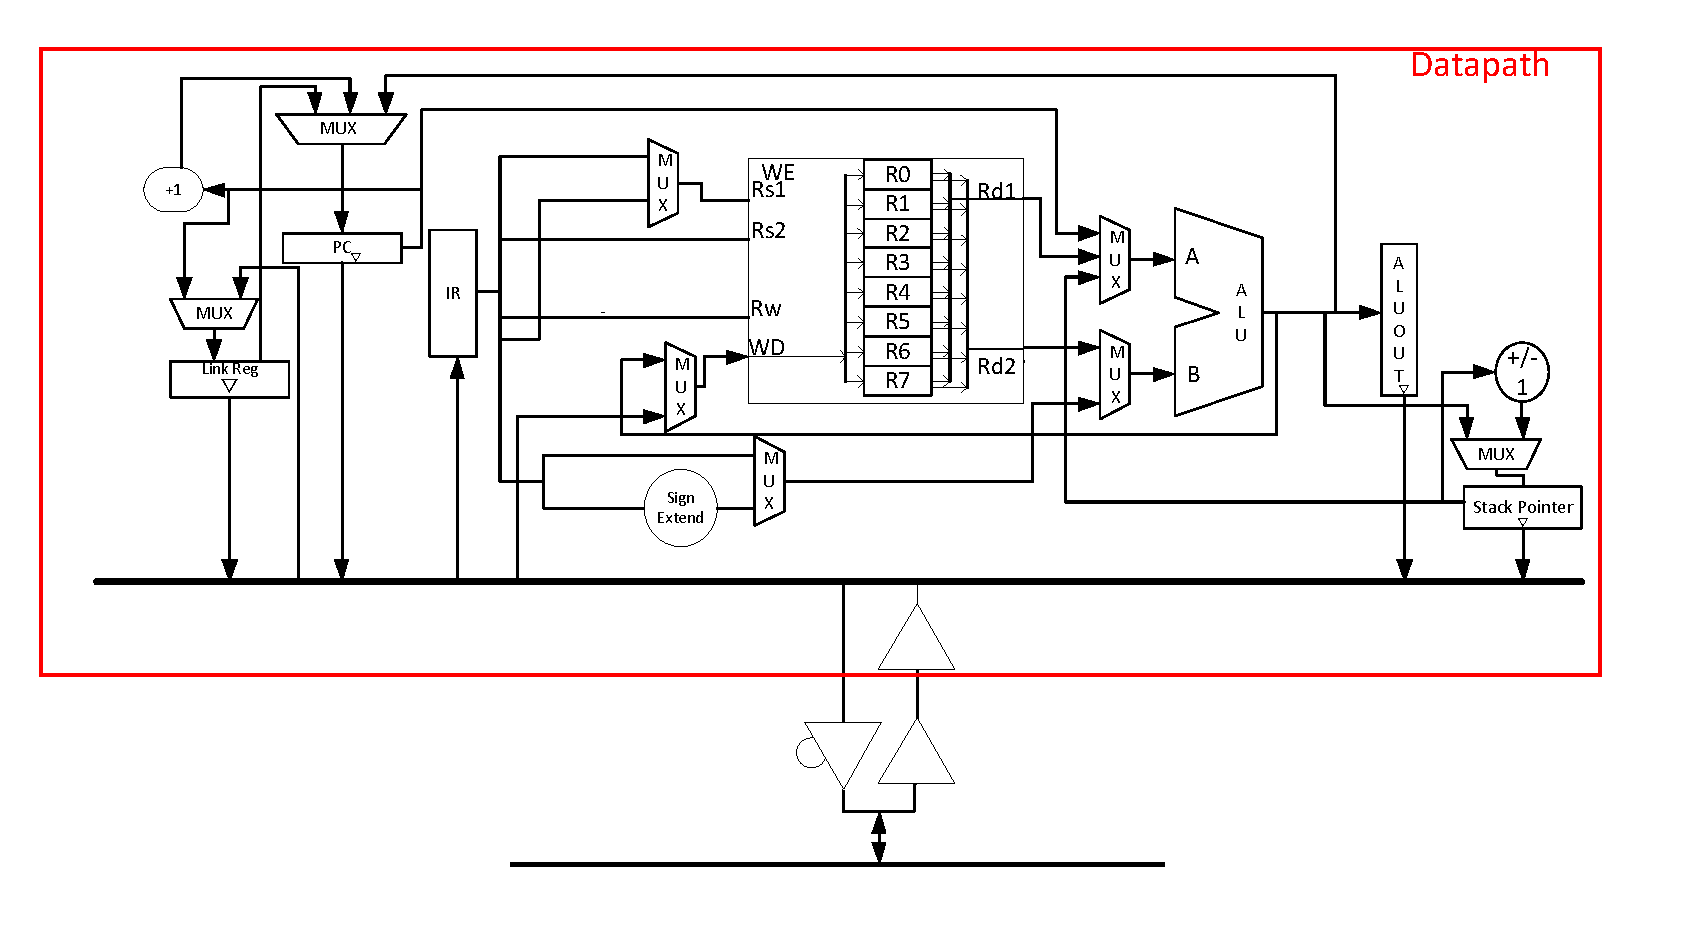
\includegraphics[angle=270,scale=0.9]{../../Design/RandD/idea1.pdf}}
}
\caption{The Architecture diagram of the processor.}
\label{fig:architecture}
\end{figure}
\todo[inline, color=green]{MW: would this need re-angling so bottom edge on outside edge of book?}


%  InstructionSet.tex
%  Date created: Thu 27 Mar 2014
%  <+Last edited: Sat 05 apr 2014 by mw20g10

\newpage
\section{Instruction Set}

The complete instruction set architecture includes a number of instructions for performing calculations on data, memory access, transfer of control\todo{HSL - this doesn't sound right. Maybe "transfer of program flow". Not sure on the use of the word "control" but i know it is the technical term} within a program and interrupt handling.\todo{HSL - this is a bit too short. Surely there is more to say about it?} 

\vspace{\baselineskip}
\noindent All instructions implemented by this architecture fall into one of 6 groups, categorized as follows:
\begin{itemize}
	\item Data Manipulation - Arithmetic, Logical, Shifting
	\item Byte Immediate - Arithmetic, Byte Load
	\item Data Transfer - Memory Access
	\item Control Transfer - (Un)conditional Branching
	\item Stack Operations - Push, Pop
	\item Interrupts - Enabling, Status Storage, Returning
\end{itemize}

\vspace{\baselineskip}
\noindent There is only one addressing mode associated with each instruction, generally following these groupings:
\begin{itemize}
	\item Data Manipulation - Register-Register, Register-Immediate
	\item Byte Immediate - Register-Immediate
	\item Data Transfer - Base Plus Offset
	\item Control Transfer - PC Relative, Register-Indirect, Base Plus Offset
	\item Stack Operations - Register-Indirect Preincrement/Postdecrement
	\item Interrupts - Register-Indirect Preincrement/Postdecrement
\end{itemize}
\vspace{\baselineskip}

\newpage

\subsection{General Instruction Formatting}
\todo[inline]{HSL - I remember Iain saying something about the instruction formats being called A1 / A2. I don't see a problem personally as I can't remember exactly what he said!}
%\newcolumntype{B}{>{\begin{varwidth}{0.2cm}} c <{\end{varwidth}}}
\newcolumntype{B}{c}
\begin{table}[h]
\centering
\footnotesize
\setlength{\tabcolsep}{2.5pt}
\makebox[\linewidth]{
\begin{tabular}{|r|l|l||BBBBBBBBBBBBBBBc|}
	 \multicolumn{1}{r}{} & \multicolumn{1}{l}{\bf Instruction Type} & \multicolumn{1}{l}{\bf Sub-Type} & 15 & 14 & 13 & 12 & 11 & 10 & 9 & 8 & 7 & 6 & 5 & 4 & 3 & 2 & 1 & \multicolumn{1}{B}{0} \\
	\hline
	A1 & \multirow{2}{*}{\bf Data Manipulation} & {\bf Register} & \multicolumn{5}{B|}{\multirow{2}{*}{Opcode}} & \multicolumn{3}{B|}{Rd} & \multicolumn{3}{B|}{Ra} & \multicolumn{3}{B|}{Rb} & X & X \\
	\cline{1-1} \cline{3-3} \cline{9-19}
	A2 &  & {\bf Immediate} & \multicolumn{5}{B|}{} & \multicolumn{3}{B|}{Rd} & \multicolumn{3}{B|}{Ra} & \multicolumn{5}{B|}{imm4/5} \\
	\hline
	B & \multicolumn{2}{l||}{\bf Byte Immediate} & \multicolumn{5}{B|}{Opcode} & \multicolumn{3}{B|}{Rd} & \multicolumn{8}{B|}{imm8} \\
	\hline
	C & \multicolumn{2}{l||}{\bf Data Transfer} & 0 & \multicolumn{1}{|B|}{LS} & 0 & 0 & \multicolumn{1}{B|}{0} & \multicolumn{3}{B|}{Rd}  &\multicolumn{3}{B|}{Ra} & \multicolumn{5}{B|}{imm5} \\
	\hline
	D1 & \multirow{2}{*}{\bf Control Transfer} & {\bf Others} & \multirow{2}{*}{1} & \multirow{2}{*}{1} & \multirow{2}{*}{1} & \multirow{2}{*}{1} & \multicolumn{1}{B|}{\multirow{2}{*}{0}} & \multicolumn{3}{B|}{\multirow{2}{*}{Cond.}}  & \multicolumn{8}{B|}{imm8} \\
	\cline{1-1} \cline{3-3} \cline{12-19}
	D2 &  & {\bf Jump} &  &  &  &  & \multicolumn{1}{B|}{} & & & \multicolumn{1}{B|}{ } & \multicolumn{3}{B|}{Ra} & \multicolumn{5}{B|}{imm5} \\
	\hline
	E & \multicolumn{2}{l||}{\bf Stack Operations} & 0 & \multicolumn{1}{|B|}{U} & 0 & 0 & \multicolumn{1}{B|}{1} & \multicolumn{1}{B|}{L} & X & \multicolumn{1}{B|}{X} & \multicolumn{3}{B|}{Ra} & 0 & 0 & 0 & 0 & \multicolumn{1}{B|}{1} \\
	\hline
	F & \multicolumn{2}{l||}{\bf Interrupts} & 1 & 1 & 0 & 0 & \multicolumn{1}{B|}{1} & \multicolumn{3}{B|}{ICond.} & 1 & 1 & \multicolumn{1}{B|}{1} & X & X & X & X & \multicolumn{1}{B|}{X} \\
	\hline
\end{tabular}
}
\end{table}
\hspace{0pt}\\\\

\begingroup
\setlength{\abovedisplayskip}{0pt}
\noindent{\bf Instruction Field Definitions} \\
\begin{alignat*}{2}
	\text{Opcode:}& \text{ Operation code as defined for each instruction} \\
	\text{Rd:}& \text{ Destination Register} \\
	\text{Ra:}& \text{ Source register 1} \\
	\text{Rb:}& \text{ Source register 2} \\
	\text{immX:}& \text{ Immediate value of length X} \\
	\text{Cond.:}& \text{ Branching condition code as defined for branch instructions} \\
	\text{ICond.:}& \text{ Interrupt instruction code as defined for interrupt instructions} \\
	\text{LS:}& \text{ 0=Load Data, 1=Store Data} \\
	\text{U:}& \text{ 1=PUSH, 0=POP} \\
	\text{L:}& \text{ 1=Use Link Register, 0=Use GPR} \\
\end{alignat*}
\endgroup

\newpage
\noindent{\bf Pseudocode Notation}
\begin{table}[h]
\centering
\footnotesize
\makebox[\linewidth]{
\begin{tabular}{|c|l|}
	\hline
	{\bf Symbol} & \multicolumn{1}{c|}{\bf Meaning} \\\hline
	$\leftarrow$, $\rightarrow$ & Assignment \\\hline
	Result[{\itshape x}] & Bit {\itshape x} of result \\\hline
	Ra[{\itshape x} : {\itshape y}] & Bit range from {\itshape x} to {\itshape y} of register Ra \\\hline
	$+Ra$ & Positive value in Register Ra \\\hline
	$-Ra$ & Negative value in Register Ra \\\hline
	\textless & Numerically greater than \\\hline
	\textgreater & Numerically less than \\\hline
	\textless\textless & Logical shift left \\\hline
	\textgreater\textgreater & Logical shift right \\\hline
	\textgreater\textgreater\textgreater & arithmetic shift right \\\hline
	Mem[{\itshape val}] & Data at memory location with address {\itshape val} \\\hline
	\{{\itshape x}, {\itshape y}\} & Contatenation of {\itshape x} and {\itshape y} to form a 16-bit value \\\hline
	({\itshape cond})? & Operation performed if {\itshape cond} evaluates to true \\\hline
	! & Bitwise Negation \\\hline
\end{tabular}
}
\end{table}\\

Use of the word UNPREDICTABLE indicates that the resultant flag value after operation execution will not be indicative of the ALU result. Instead its value will correspond to the result of an undefined arithmetic operation and as such should not be used. 

%
% Instructions 1-8
%
\Imnemonic{Add Word}{ADD}
\Iformat{A}{00010}
\Isyntax{ADD Rd, Ra, Rb}{ADD R5, R3, R2}
\Ioperation{Rd $\leftarrow$}{Ra + Rb}{C}{V}{b}{0}{N}{Z}
\Idesc{The 16-bit word in GPR[Ra] is added to the 16-bit word in GPR[Rb] and the result is placed into GPR[Rd]. \\\\ Addressing Mode: Register-Register.}
\newpage
\Imnemonic{Add Immediate}{ADDI}
\Iformat{a}{00110}
\Isyntax{ADDI Rd, Ra, \#imm5}{ADDI R5, R3, \#7}
\Ioperation{Rd $\leftarrow$}{Ra + \#imm5}{C}{V}{5}{0}{N}{Z}
\Idesc{The 16-bit word in GPR[Ra] is added to the sign-extended 5-bit value given in the instruction and the result is placed into GPR[Rd]. \\\\ Addressing Mode: Register-Immediate.}
\newpage
\Imnemonic{Add Immediate Byte}{ADDIB}
\Iformat{B}{00011}
\Isyntax{ADDIB Rd, \#imm8}{ADDIB R5, \#93}
\Ioperation{Rd $\leftarrow$}{Rd + \#imm8}{C}{V}{8}{0}{N}{Z}
\Idesc{The 16-bit word in GPR[Rd] is added to the sign-extended 8-bit value given in the instruction and the result is placed into GPR[Rd]. \\\\ Addressing Mode: Register-Immediate.}
\newpage
\Imnemonic{Add Word With Carry}{ADC}
\Iformat{A}{00100}
\Isyntax{ADC Rd, Ra, Rb}{ADC R5, R3, R2}
\Ioperation{Rd $\leftarrow$}{Ra + Rb + C}{C}{V}{b}{c}{N}{Z}
\Idesc{The 16-bit word in GPR[Ra] is added to the 16-bit word in GPR[Rb] with the added carry in set according to the Carry flag from previous operation, and the result is placed into GPR[Rd]. \\\\ Addressing Mode: Register-Register.}
\newpage
\Imnemonic{Add Immediate With Carry}{ADCI}
\Iformat{a}{00101}
\Isyntax{ADCI Rd, Ra, \#imm5}{ADCI R5, R4, \#7}
\Ioperation{Rd $\leftarrow$}{Ra + \#imm5 + C}{C}{V}{5}{c}{N}{Z}
\Idesc{The 16-bit word in GPR[Ra] is added to the sign-extended 5-bit value given in the instruction with carry in set according to the Carry flag from previous operation, and the result is placed into GPR[Rd]. \\\\ Addressing Mode: Register-Immediate.}
\newpage
\Imnemonic{Negate Word}{NEG}
\Iformat{A}{11010}
\Isyntax{NEG Rd, Ra}{NEG R5, R3}
\Ioperation{Rd $\leftarrow$}{0 - Ra}{C}{V}{b}{0}{N}{Z}
\Idesc{The 16-bit word in GPR[Ra] is added to the 16-bit word in GPR[Rb] and the result is placed into GPR[Rd]. \\\\ Addressing Mode: Register-Register.}
\newpage
\Imnemonic{Subtract Word}{SUB}
\Iformat{A}{01010}
\Isyntax{SUB Rd, Ra, Rb}{SUB R5, R3, R2}
\Ioperation{Rd $\leftarrow$}{Ra - Rb}{C}{V}{b}{0}{N}{Z}
\Idesc{The 16-bit word in GPR[Rb] is subtracted from the 16-bit word in GPR[Ra] and the result is placed into GPR[Rd]. \\\\ Addressing Mode: Register-Register.}
\newpage
\Imnemonic{Subtract Immediate}{SUBI}
\Iformat{a}{01110}
\Isyntax{SUBI Rd, Ra, \#imm5}{SUBI R5, R3, \#7}
\Ioperation{Rd $\leftarrow$}{Ra - \#imm5}{C}{V}{5}{0}{N}{Z}
\Idesc{The sign extended 5-bit value given in the instruction is subtracted from the 16-bit word in GPR[Ra] and the result is placed into GPR[Rd]. \\\\ Addressing Mode: Register-Immediate.}
\newpage
%
% Instructions 9-16
%
\Imnemonic{Subtract Immediate Byte}{SUBIB}
\Iformat{B}{01011}
\Isyntax{SUBIB Rd, \#imm8}{SUBIB R5, \#93}
\Ioperation{Rd $\leftarrow$}{Rd - \#imm8}{C}{V}{8}{0}{N}{Z}
\Idesc{The 8-bit immediate value given in the instruction is subtracted from the 16-bit word in GPR[Rd] and the result is placed into GPR[Rd]. \\\\ Addressing Mode: Register-Immediate.}
\newpage
\Imnemonic{Subtract Word With Carry}{SUC}
\Iformat{A}{01100}
\Isyntax{SUC Rd, Ra, Rb}{SUC R5, R3, R2}
\Ioperation{Rd $\leftarrow$}{Ra - Rb - C}{C}{V}{b}{n}{N}{Z}
\Idesc{The 16-bit word in GPR[Rb] is subtracted from the 16-bit word in GPR[Rb] with the subtracted carry in set according to the Carry flag from previous operation, and the result is placed into GPR[Rd]. \\\\ Addressing Mode: Register-Register.}
\newpage
\Imnemonic{Subtract Immediate With Carry}{SUCI}
\Iformat{a}{01101}
\Isyntax{SUCI Rd, Ra, \#imm5}{SUCI R5, R4, \#7}
\Ioperation{Rd $\leftarrow$}{Ra - \#imm5 - C}{C}{V}{5}{n}{N}{Z}
\Idesc{The 5-bit immediate value in instruction is subtracted from the 16-bit word in GPR[Ra] with the subtracted carry in set according to the Carry flag from previous operation, and the result is placed into GPR[Rd]. \\\\ Addressing Mode: Register-Immediate.}
\newpage
\Imnemonic{Compare Word}{CMP}
\Iformat{A}{00111}
\Isyntax{CMP Ra, Rb}{CMP R3, R2}
\Ioperation{X}{Ra - Rb}{C}{V}{b}{0}{N}{Z}
\Idesc{The 16-bit word in GPR[Rb] is subtracted from the 16-bit word in GPR[Ra] and the status flags are updated without saving the result. \\\\ Addressing Mode: Register-Register.}
\newpage
\Imnemonic{Compare Immediate}{CMPI}
\Iformat{a}{01111}
\Isyntax{CMPI Ra, \#imm5}{CMPI R3, \#7}
\Ioperation{X}{Ra - \#imm5}{C}{V}{5}{0}{N}{Z}
\Idesc{The sign extended 5-bit value given in the instruction is subtracted from the 16-bit word in GPR[Ra] and the status flags are updated without saving the result. \\\\ Addressing Mode: Register-Immediate.}
\newpage
\Imnemonic{Logical AND}{AND}
\Iformat{A}{10000}
\Isyntax{AND Rd, Ra, Rb}{AND R5, R3, R2}
\Ioperation{Rd $\leftarrow$}{Ra AND Rb}{U}{U}{0}{0}{N}{Z}
\Idesc{The logical AND of the 16-bit words in GPR[Ra] and GPR[Rb] is performed and the result is placed into GPR[Rd]. \\\\ Addressing Mode: Register-Register.}
\newpage
\Imnemonic{Logical OR}{OR}
\Iformat{A}{10001}
\Isyntax{OR Rd, Ra, Rb}{OR R5, R3, R2}
\Ioperation{Rd $\leftarrow$}{Ra OR Rb}{U}{U}{0}{0}{N}{Z}
\Idesc{The logical OR of the 16-bit words in GPR[Ra] and GPR[Rb] is performed and the result is placed into GPR[Rd]. \\\\ Addressing Mode: Register-Register.}
\newpage
\Imnemonic{Logical XOR}{XOR}
\Iformat{A}{10011}
\Isyntax{XOR Rd, Ra, Rb}{XOR R5, R3, R2}
\Ioperation{Rd $\leftarrow$}{Ra XOR Rb}{U}{U}{0}{0}{N}{Z}
\Idesc{The logical XOR of the 16-bit words in GPR[Ra] and GPR[Rb] is performed and the result is placed into GPR[Rd]. \\\\ Addressing Mode: Register-Register.}
\newpage
%
% Instructions 17-24
%
\Imnemonic{Logical NOT}{NOT}
\Iformat{A}{10010}
\Isyntax{NOT Rd, Ra}{NOT R5, R3}
\Ioperation{Rd $\leftarrow$}{NOT Ra}{U}{U}{0}{0}{N}{Z}
\Idesc{The logical NOT of the 16-bit word in GPR[Ra] is performed and the result is placed into GPR[Rd]. \\\\ Addressing Mode: Register-Register.}
\newpage
\Imnemonic{Logical NAND}{NAND}
\Iformat{A}{10110}
\Isyntax{NAND Rd, Ra, Rb}{NAND R5, R3, R2}
\Ioperation{Rd $\leftarrow$}{Ra NAND Rb}{U}{U}{0}{0}{N}{Z}
\Idesc{The logical NAND of the 16-bit words in GPR[Ra] and GPR[Rb] is performed and the result is placed into GPR[Rd]. \\\\ Addressing Mode: Register-Register.}
\newpage
\Imnemonic{Logical NOR}{NOR}
\Iformat{A}{10111}
\Isyntax{NOR Rd, Ra, Rb}{NOR R5, R3, R2}
\Ioperation{Rd $\leftarrow$}{Ra NOR Rb}{U}{U}{0}{0}{N}{Z}
\Idesc{The logical NOR of the 16-bit words in GPR[Ra] and GPR[Rb] is performed and the result is placed into GPR[Rd]. \\\\ Addressing Mode: Register-Register.}
\newpage
\Imnemonic{Logical Shift Left}{LSL}
\Iformat[s]{a}{11111}
\Isyntax{LSL Rd, Ra, \#imm4}{LSL R5, R3, \#7}
\Ioperation{Rd $\leftarrow$}{Ra $<<$ \#imm4}{U}{U}{0}{0}{N}{Z}
\Idesc{The 16-bit word in GPR[Ra] is shifted left by the 4-bit amount specified in the instruction, shifting in zeros, and the result is placed into GPR[Rd]. \\\\ Addressing Mode: Register-Immediate.}
\newpage
\Imnemonic{Logical Shift Right}{LSR}
\Iformat[s]{a}{11101}
\Isyntax{LSR Rd, Ra, \#imm4}{LSR R5, R3, \#7}
\Ioperation{Rd $\leftarrow$}{Ra $>>$ \#imm4}{U}{U}{0}{0}{N}{Z}
\Idesc{The 16-bit word in GPR[Ra] is shifted right by the 4-bit amount specified in the instruction, shifting in zeros, and the result is placed into GPR[Rd]. \\\\ Addressing Mode: Register-Immediate.}
\newpage
\Imnemonic{Arithmetic Shift Right}{ASR}
\Iformat[s]{a}{11100}
\Isyntax{ASR Rd, Ra, \#imm4}{ASR R5, R3, \#7}
\Ioperation{Rd $\leftarrow$}{Ra $>>>$ \#imm4}{U}{U}{0}{0}{N}{Z}
\Idesc{The 16-bit word in GPR[Ra] is shifted right by the 4-bit amount specified in the instruction, shifting in the sign bit of Ra, and the result is placed into GPR[Rd]. \\\\ Addressing Mode: Register-Immediate.}
\newpage
\Imnemonic{Load Word}{LDW}
\Iformat{C}{0}
\Isyntax{LDW Rd, [Ra, \#imm5]}{LDW R5, [R3, \#7]}
\Ioperation{Rd $\leftarrow$}{Mem[Ra + \#imm5]}{n}{n}{5}{0}{n}{n}
\Idesc{Data is loaded from memory at the resultant address from addition of GPR[Ra] and the 5-bit immediate value specified in the instruction, and the result is placed into GPR[Rd]. \\\\ Addressing Mode: Base Plus Offset.}
\newpage
\Imnemonic{Store Word}{STW}
\Iformat{C}{1}
\Isyntax{STW Rd, [Ra, \#imm5]}{STW R5, [R3, \#7]}
\Ioperation{Mem}{[Ra + \#imm5] $\leftarrow$ Rd}{n}{n}{5}{0}{n}{n}
\Idesc{Data in GPR[Rd] is stored to memory at the resultant address from addition of GPR[Ra] and the 5-bit immediate value specified in the instruction. \\\\ Addressing Mode: Base Plus Offset.}
\newpage
%
% Instructions 25-32
%
\Imnemonic{Load Upper Immediate}{LUI}
\Iformat{B}{10100}
\Isyntax{LUI Rd \#imm8}{LUI R5, \#93}
\Ioperation{Rd $\leftarrow$}{\{\#imm8,~0\}}{n}{n}{0}{0}{n}{n}
\Idesc{The 8-bit immediate value provided in the instruction is loaded into the top half in GPR[Rd], setting the bottom half to zero. \\\\ Addressing Mode: Register-Immediate.}
\newpage
\Imnemonic{Load Lower Immediate}{LLI}
\Iformat{B}{10101}
\Isyntax{LLI Rd \#imm8}{LLI R5, \#93}
\Ioperation{Rd $\leftarrow$}{\{Rd[15:8],~\#imm8\}}{n}{n}{0}{0}{n}{n}
\Idesc{The 8-bit immediate value provided in the instruction is loaded into the bottom half in GPR[Rd], leaving the top half unchanged. \\\\ Addressing Mode: Register-Immediate.}
\newpage
\Imnemonic{Branch Always}{BR}
\Iformat{D}{000}
\Isyntax{BR LABEL}{BR .loop}
\Ioperation{PC $\leftarrow$}{PC + \#imm8}{n}{n}{8}{0}{n}{n}
\Idesc{Unconditionally branch to the resultant address from addition of PC and the 8-bit immediate value specified in the instruction. LABEL can be both a symbolic name or a numeric value, and is capable of jumping forwards or backwards.\\\\ Addressing Mode: PC Relative.}
\newpage
\Imnemonic{Branch If Not Equal}{BNE}
\Iformat{D}{110}
\Isyntax{BNE LABEL}{BNE .loop}
\Ioperation{PC $\leftarrow$}{PC + \#imm8~(z==0)?}{n}{n}{8}{0}{n}{n}
\Idesc{Conditionally branch to the resultant address from addition of PC and the 8-bit immediate value specified in the instruction if zero status flag (Z) equals zero. LABEL can be both a symbolic name or a numeric value, and is capable of jumping forwards or backwards.\\\\ Addressing Mode: PC Relative.}
\newpage
\Imnemonic{Branch If Equal}{BE}
\Iformat{D}{111}
\Isyntax{BE LABEL}{BE .loop}
\Ioperation{PC $\leftarrow$}{PC + \#imm8~(z==1)?}{n}{n}{8}{0}{n}{n}
\Idesc{Conditionally branch to the resultant address from addition of PC and the 8-bit immediate value specified in the instruction if zero status flag (Z) equals one. LABEL can be both a symbolic name or a numeric value, and is capable of jumping forwards or backwards.\\\\ Addressing Mode: PC Relative.}
\newpage
\Imnemonic{Branch If Less Than}{BLT}
\Iformat{D}{100}
\Isyntax{BLT LABEL}{BLT .loop}
\Ioperation{PC $\leftarrow$}{PC + \#imm8~(n\&!v~OR~!n\&v)?}{n}{n}{8}{0}{n}{n}
\Idesc{Conditionally branch to the resultant address from addition of PC and the 8-bit immediate value specified in the instruction if negative status flag and overflow status flag are not equivalent. LABEL can be both a symbolic name or a numeric value, and is capable of jumping forwards or backwards.\\\\ Addressing Mode: PC Relative.}
\newpage
\Imnemonic{Branch If Greater Than Or Equal}{BGE}
\Iformat{D}{101}
\Isyntax{BGE LABEL}{BGE .loop}
\Ioperation{PC $\leftarrow$}{PC + \#imm8~(n\&v~OR~!n\&!v)?}{n}{n}{8}{0}{n}{n}
\Idesc{Conditionally branch to the resultant address from addition of PC and the 8-bit immediate value specified in the instruction if negative status flag and overflow status flag are equivalent. LABEL can be both a symbolic name or a numeric value, and is capable of jumping forwards or backwards.\\\\ Addressing Mode: PC Relative.}
\newpage
\Imnemonic{Branch With Link}{BWL}
\Iformat{D}{011}
\Isyntax{BWL LABEL}{BWL .loop}
\Ioperation{LR $\leftarrow$}{PC + 1;~PC $\leftarrow$ PC + \#imm8}{n}{n}{8}{0}{n}{n}
\Idesc{Save the current program counter (PC) value plus one to the link register. Then unconditionally branch to the resultant address from addition of PC and the 8-bit immediate value specified in the instruction. LABEL can be both a symbolic name or a numeric value, and is capable of jumping forwards or backwards.\\\\ Addressing Mode: PC Relative.}
\newpage
%
% Instructions 33-40
%
\Imnemonic{Return}{RET}
\Iformat{D}{010}
\Isyntax{RET}{RET}
\Ioperation{PC $\leftarrow$}{LR}{n}{n}{0}{0}{n}{n}
\Idesc{Unconditionally branch to the address stored in the link register (LR).\\\\ Addressing Mode: Register-Indirect.}
\newpage
\Imnemonic{Jump}{JMP}
\Iformat{D}{001}
\Isyntax{JMP Ra, \#imm5}{JMP R3, \#7}
\Ioperation{PC $\leftarrow$}{Ra + \#imm5}{n}{n}{8}{0}{n}{n}
\Idesc{Unconditionally jump to the resultant address from the addition of GPR[Ra] and the 5-bit immediate value specified in the instruction.\\\\ Addressing Mode: Base Plus Offset.}
\newpage
\Imnemonic{Push From Stack}{PUSH}
\Iformat{E}{1L0}
\Isyntax[M]{PUSH Ra}{PUSH R3}
\Isyntax[F]{PUSH RL}{PUSH RL}
\Ioperation{Mem}{[R7] $\leftarrow$ reg; R7 $\leftarrow$ R7 - 1}{n}{n}{0}{0}{n}{n}
\Idesc{`reg' corresponds to either a GPR or the link register, the contents of which are stored to the stack using the address stored in the stack pointer (R7). Then Decrement the stack pointer by one. \\\\Addressing Modes: Register-Indirect, Postdecrement.}
\newpage
\Imnemonic{Pop From Stack}{POP}
\Iformat{E}{0L}
\Isyntax[M]{POP Ra}{POP R3}
\Isyntax[F]{POP RL}{POP RL}
\Ioperation{R7 $\leftarrow$}{R7 + 1; Mem[R7] $\leftarrow$ reg;}{n}{n}{0}{0}{n}{n}
\Idesc{Increment the stack pointer by one. Then `reg' corresponds to either a GPR or the link register, the contents of which are retrieved from the stack using the address stored in the stack pointer (R7). \\\\Addressing Modes: Register-Indirect, Preincrement.}
\newpage
\Imnemonic{Return From Interrupt}{RETI}
\Iformat{F}{000}
\Isyntax{RETI}{RETI}
\Ioperation{PC $\leftarrow$}{Mem[R7]}{n}{n}{0}{0}{n}{n}
\Idesc{Restore program counter to its value before interrupt occured, which is stored on the stack, pointed to be the stack pointer (R7). This must be the last instruction in an interrupt service routine. \\\\ Addressing Mode: Register-Indirect.}
\newpage
\Imnemonic{Enable Interrupts}{ENAI}
\Iformat{F}{001}
\Isyntax{ENAI}{ENAI}
\Ioperation{Set }{Interrupt Enable Flag}{n}{n}{0}{0}{n}{n}
\Idesc{Turn on interrupts by setting interrupt enable flag to true (1).}
\newpage
\Imnemonic{Disable Interrupts}{DISI}
\Iformat{F}{010}
\Isyntax{DISI}{DISI}
\Ioperation{Reset}{ Interrupt Enable Flag}{n}{n}{0}{0}{n}{n}
\Idesc{Turn off interrupts by setting interrupt enable flag to false (0).}
\newpage
\Imnemonic{Store Status Flags}{STF}
\Iformat{F}{011}
\Isyntax{STF}{STF}
\Ioperation{Mem}{[R7] $\leftarrow$ \{12-bit 0, Z, C, V, N\}; R7 $\leftarrow$ R7 - 1;}{n}{n}{0}{0}{n}{n}
\Idesc{Store contents of status flags to stack using address held in stack pointer (R7). Then decrement the stack pointer (R7) by one. \\\\  Addressing Modes: Register-Indirect, Postdecrement.}
\newpage
%
% Instruction 41
%
\Imnemonic{Load Status Flags}{LDF}
\Iformat{F}{100}
\Isyntax{LDF}{LDF}
%\Ioperation{R7 $\leftarrow$}{R7 + 1; \{Z, C, V, N\} $\leftarrow$ Mem[R7][3:0]}{0}{0}{0}{0}{0}{0}
\begingroup
	\setlength{\tabcolsep}{2pt}
	\indent\textbf{Operation} \\
	\indent\indent
	\begin{tabular}{rl}
		R7 $\leftarrow$& R7 + 1 \\
		\phantom{R} N $\leftarrow$& Mem[R7][0] \\
		Z $\leftarrow$& Mem[R7][3] \\
		V $\leftarrow$& Mem[R7][1] \\
		C $\leftarrow$& Mem[R7][2] \\\\\\
	\end{tabular}
	\\\\	
	\endgroup
\Idesc{Increment the stack pointer (R7) by one. Then load content of status flags with lower 4 bits of value retrieved from stack using address held in stack pointer (R7). \\\\ Addressing Modes: Register-Indirect, Preincrement.}
\newpage

%  Implementation.tex
%  Document created by seblovett on seblovett-Ubuntu
%  Date created: Thu 17 Apr 2014 15:12:30 BST
%  <+Last Edited: Thu 17 Apr 2014 15:37:15 BST by seblovett on seblovett-Ubuntu +>


\chapter{Design and Implementation}

%  Register_Design.tex
%  Document created by seblovett on seblovett-Ubuntu
%  Date created: Thu 17 Apr 2014 14:59:55 BST
%  <+Last Edited: Sun 11 May 2014 15:16:13 BST by seblovett on seblovett-Ubuntu +>

\section{Register Block}

%Design of whole module, including circuit diagram
The register block contains eight general purpose registers. 
No dummy register is implemented in the register block. 
The module has three address inputs, two read addresses and one write address. 
There are two read outputs, which output the stored data, and a data input to be written. 
Reads are asynchronous and must always be driven. 
Writes are synchronous and must implement a write enable signal. 

%Use of hierarchy / blocks - i.e. bit sliced, decoder
To optimise the design for space, the module is broken down into a bit slice and a decoder. 
The whole block is made up of sixteen slices and one decoder. 

\subsection{Bit Slice Design}

The bit slice consists of eight load enable registers. 
Two tristate buffers are used per register onto different buses for the two read data outputs. 
The registers are selected by one hot coding and as such will result in the output bus always being driven. 
The write enables are also controlled using one hot coding. 
However, all signals are allowed to be off if no register is to be written to.
The circuit diagram for the bit slice is seen in Figure~\ref{fig:reg:slice}.

\begin{figure}
\centering
\includegraphics[angle=90,height=\textheight]{../../eagle/regBlock/regBlock_slice.png}
\caption{Circuit diagram for the register block slice.}
\label{fig:reg:slice}
\end{figure}



\begin{table}
\caption{Decoder Logic Functions}
\label{tab:reg:decoder}
\centering
\begin{tabular}{cc}
Register Number & Logic Select Function \\
0		&		$!( Rs0 | Rs1 | Rs2 )$ \\
1		&		$ !( Rs1 | Rs2 ) \& Rs0$	\\
2		&		$!( Rs2 | Rs0 ) \& Rs1$\\
3		&		$! ( ! ( Rs0 \& Rs1 ) | Rs2 )$	\\
4		&		$!( Rs0 | Rs1 ) \& Rs2$	\\
5		&		$! ( ! ( Rs0 \& Rs2 ) | Rs1 )$	\\
6		&		$! ( ! ( Rs1 \& Rs2 ) | Rs0 )$	\\
7		&		$Rs0 \& Rs1 \& Rs2$	\\
\end{tabular}

\end{table}

The read decoder is based around a 3-8 decoder. 
For each 3 bit input, one and only one output should be high. 
The logic functions used are summarised in Table~\ref{tab:reg:decoder}.
The bit sliced circuit diagram is shown in Figure~\ref{fig:reg:decoder}.
This illustrates only one of the decoders needed since the second is identical.
However, the write decoder must also use a write enable signal.
This is done by using the same logic functions shown in Table~\ref{tab:reg:decoder}, but the resulting signals are then \texttt{AND}ed with the register write enable signal. 
%\todo[inline, color=green]{MW: Ive re-worded this a bit}
%\todo[inline, color=green]{MW: what do you mean by write enable function?}

\begin{figure}
\centering
%\missingfigure{Decoder circuit diagram}
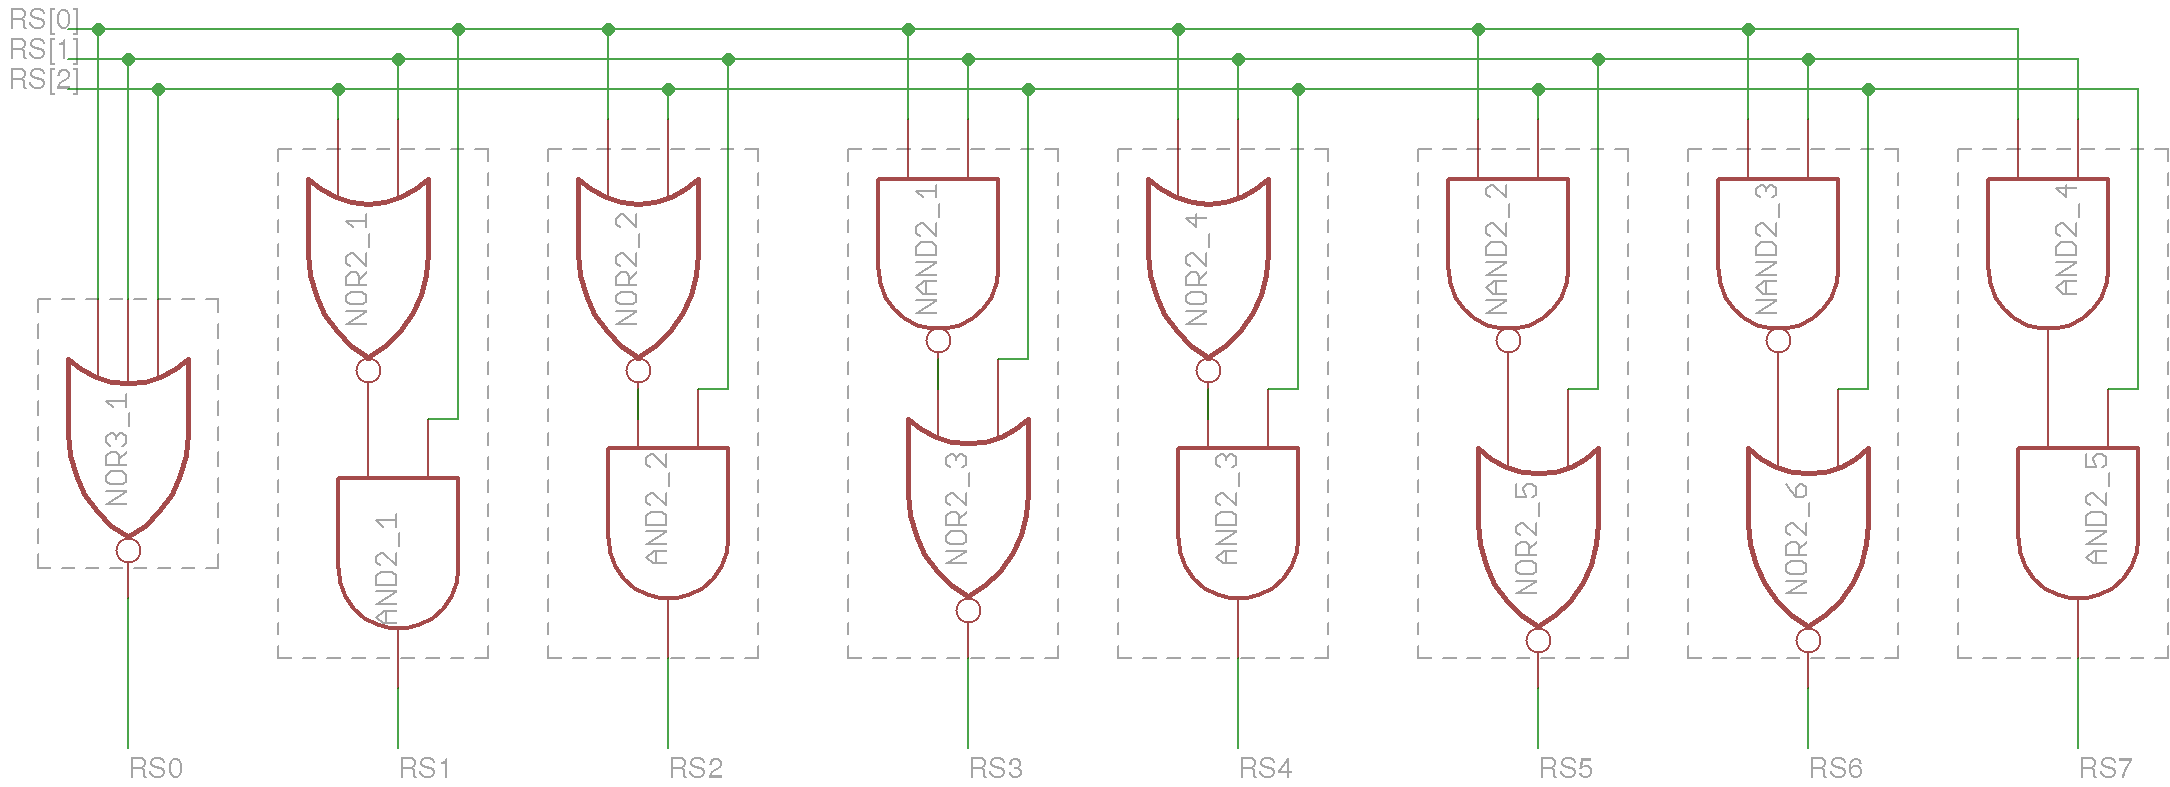
\includegraphics[width=\textwidth]{../../eagle/regBlock/regBlock_decoder.png}
\caption{Circuit diagram for the register decoder.}
\label{fig:reg:decoder}
\end{figure}
%Design of block,

%Layout in silicon
The layout in silicon consisted of an array of slices. 
All I/Os for the slice are then in the same position and all global signals from the decoder are propagated through the slice.
The use of tristate buffers reduces the wiring needed in the design. 
The decoder was designed to fit above the block of general purpose registers. 
All three decoders were distributed in the implementation and spaced to reduce the size of the wiring channel.
%\todo[inline, color=green]{MW: which buffers? HSL: what? MW:I forgot what that means}

%  PC_Design.tex
%  Document created by seblovett on seblovett-Ubuntu
%  Date created: Thu 17 Apr 2014 15:01:32 BST
%  <+Last Edited: Sun 11 May 2014 20:21:14 BST by seblovett on seblovett-Ubuntu +>

\section{Program Counter and Link Register}


%Design of whole module, including circuit diagram
The program counter and link register were implemented in one module.
The module has two load enable registers. 
The data source logic and an adder for incrementing the program counter is also implemented in this module.

The program counter sources are:
\begin{enumerate}
\item Incremented program counter - for normal sequential operation
\item Link Register - for returning from a subroutine call
\item ALU output - for a jump to a register contents
\item System bus - for returning the program counter from the stack after an interrupt service routine.
\item ISR Location - a constant defined for the location of the interrupt service routine in memory.
\end{enumerate}

The link register has two inputs:
\begin{enumerate}
\item Incremented program counter - for storing the return address when executing a function call
\item System Bus - for retrieving a return address from the stack 
\end{enumerate}

%Use of hierarchy / blocks - i.e. bit sliced, decoder
This module is made up of sixteen identical bitslices. 
All control signals are connected to the controller and so no decoder is needed in this module.
The circuit diagram is shown in Figure~\ref{fig:pc:circuit}.
%Design of slice,
The slice is implemented to match the circuit diagram. 
%Multiplexors are used instead of tristate buffers as there is little wiring involved. 
Multiplexors are used instead of tristate buffers since there are few data sources used which are not significantly distributed around the datapath to require a bus. 
It also removes the need for a decoder.
%\todo[inline, color=green]{MW:Some of this is surely implied, could you not say more? @seblovett; HSL: It's a very simple module, not much to say here really. MW:Guess its hard to expand}

\begin{figure}
\centering
\includegraphics[width=\textwidth-2.7cm]{../../eagle/PcBlock/PcBlock_slice.png}
\caption{Circuit Diagram for Program Counter and Link Register block slice.}
\label{fig:pc:circuit}
\end{figure}

%Design of block,
The module is made up of an array of slices. 
The control signals are propagated throughout the module vertically. 
The system bus connection has also been added and the carry out and the second input to the half adder must be connected between the slices.

%  IR_Design.tex
%  Document created by seblovett on seblovett-Ubuntu
%  Date created: Thu 17 Apr 2014 15:01:50 BST
%  <+Last Edited: Sun 11 May 2014 15:18:54 BST by seblovett on seblovett-Ubuntu +>

\section{Instruction Register}


%Design of whole module, including circuit diagram
The instruction register module has a load enable register for storing of the instruction.
It also has the immediate selection and sign extension circuitry.
The two immediate values are either a five bit signed value located at position [4:0] of the instruction, or an eight bit signed value at [7:0] of the instruction.
Only the \textbf{LLI} instruction does not use a signed immediate value. 
This is implemented by the ALU, discussed in Section~\ref{sect:design:alu}.
%The ALU therefore ignores the top eight bits of the immediate value. 
%ALU design is discussed further in Section~\ref{sect:design:alu}.
%\todo[inline, color=green]{MW: Is ALU comment needed as it is discussed later?}


%Use of hierarchy / blocks - i.e. bit sliced, decoder
The instruction register module is separated into three different bit slices.
The circuit diagrams for these are shown in Figure~\ref{fig:ir:circuit}.
It cannot be broken into sixteen identical modules due to data in the instruction needing sign extension. 

The data for the instruction register is only read from the system bus. 
The instruction is then directly fed out of this module to the controller or register decoding blocks.
The three blocks differ due to the sign extension and are referred to as ``AA'', ``BA'' or ``BB''.
The three modules contain the same cells, but the input and output wires to the multiplexor differ. 
\begin{enumerate}
\item[BB] - This block takes the value of the instruction register and passes it to both of the multiplexor inputs. The multiplexor is redundant here but kept to keep the sizes of the three modules identical. All inputs to the bottom of this module are ignored.
\item[BA] - This block chooses between the instruction register value or a value passed into the bottom of the module. This input is the sign of the five bit immediate and is outputted to the top of the module.
\item[AA] - The final block chooses the sign from either the eight or five bit immediate. The signs are passed in at the bottom of the module and propagated to the top. 
\end{enumerate}

By stacking these modules using $5\times$BB, $3\times$BA and $8\times$AA (bottom to top), the sign bits will be propagated at the correct points.
The output is then a full sixteen bit signed value of the relevant immediate selected by the \textit{ImmSel} signal.
\begin{figure}
\centering
\subfloat[The AA type slice]{\label{fig:ir:circuit:aa}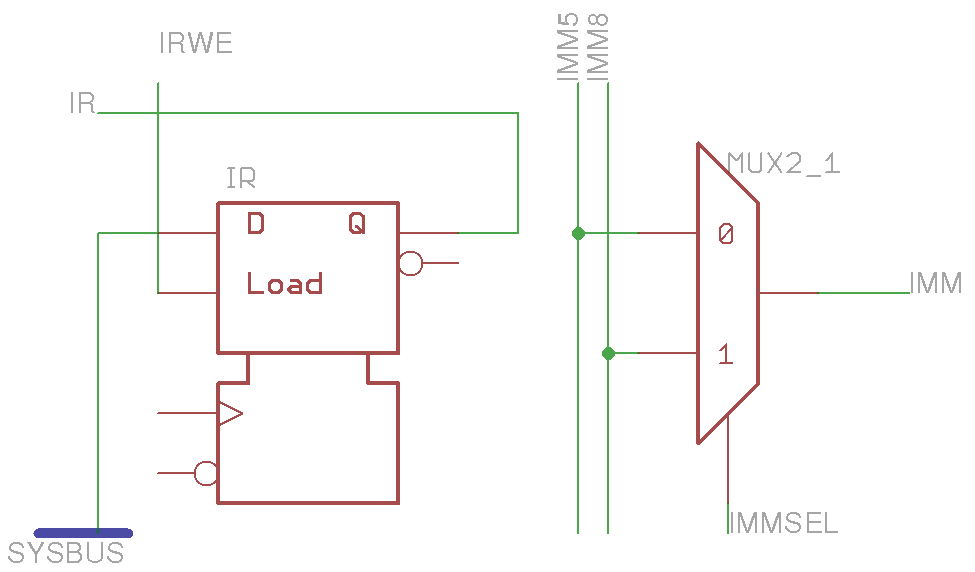
\includegraphics[width=0.5\textwidth]{../../eagle/Ir/IrAA.png}}
\subfloat[The BA type slice]{\label{fig:ir:circuit:ba}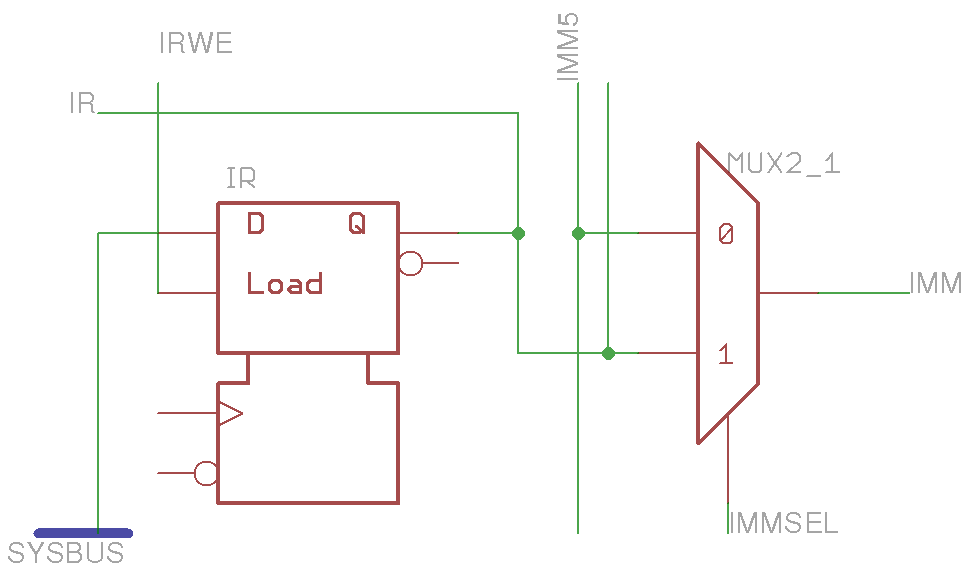
\includegraphics[width=0.5\textwidth]{../../eagle/Ir/IrBA.png}}\\
\subfloat[The BB type slice]{\label{fig:ir:circuit:bb}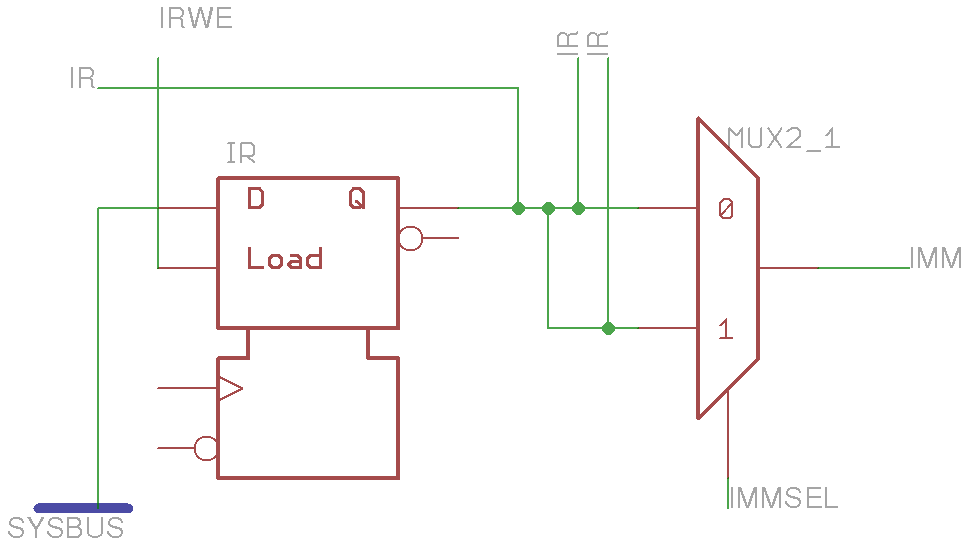
\includegraphics[width=0.5\textwidth]{../../eagle/Ir/IrBB.png}}
\caption{The three circuits used for the instruction register block.}
\label{fig:ir:circuit}
\end{figure}



%  ALU_Design.tex
%  Document created by seblovett on seblovett-Ubuntu
%  Date created: Thu 17 Apr 2014 15:00:33 BST
%  <+Last Edited: Mon 05 May 2014 11:39:09 BST by seblovett on seblovett-Ubuntu +>


\section{Arithmetic Logic Unit}\label{sect:design:alu}
\todo[color=cyan, inline]{Design of whole module - ongoing}
\todo[color=cyan, inline]{Use of hierarchy - implied mention, todo}
\todo[color=cyan, inline]{Design of slice - initial text done}
\todo[color=cyan, inline]{Design of decoder - initial text done}
\todo[color=cyan, inline]{Design of block - initial test done}
\todo[color=cyan, inline]{Layout in silicon}

The arithmetic logic unit (ALU) is the central unit for performing calculations within the datapath. 
Most instructions use the ALU as part of their operation and as such this module needs to interpret every instruction and perform the necessary function. 
The range of functions needed fall into one of four types: arithmetic, logic, shifting and load lower. 
With the last type being a special case for the LLI instruction. 
Arithmetic operations are centralized around a full adder with additional gates for subtraction, setting the first input to zero and flag calculations. 
The logic unit consists of one gate corresponding to each of the full set of logic instructions supported. 
While shifts are performed using a barrel shifter to support up to 15-bits in one clock cycle. 
Finally, the LLI module concatenates the upper byte of the destination register with the provided 8-bit immediate value. 
The breakdown of the ALU is illustrated in Figure~\ref{fig:abstractALU}, with the output of each section connected to an internal bus through a number of tri-state gates. 


\begin{figure}[h]
	\missingfigure{Abstract ALU Breakdown}
	\caption{ALU Separated into Sub-modules}
	\label{fig:abstractALU}
\end{figure}

This design then needed to be bit-sliced to simplify the datapath and promote hierarchical construction. 
It was decided to add an additional input to the module for the 4-bit immediate value required to define the shifting amount. 
Otherwise the lowest four bits of the ALU will each need a different routing to each segment, reducing how much of each slice could be identically duplicated. 
\todo[inline,color=green]{HSL - @MW tenses change in this. Should be past - ``it was designed in bit slices\dots''}

Initial design of the ALU module was based upon the planned datapath layout and the input/output connections it showed, as seen in Figure~\ref{fig:BasicALUSym}. 
From this it was seen that there may be some difficulty with interpreting the opcodes provided. 
Since each slice would have to individually interpret the opcode, using much more space than is necessary due to replicated hardware. 
Observations showed that different groups of instructions would perform the same operation within the ALU. 
As such, it was decided to use a separate decoder to interpret the opcodes and send control lines to the ALU for the specific functions to be performed. 
\todo[inline,color=green]{HSL - @MW - I don't think this aids to any understanding. 
The final point is key, but could be condensed down into one/two lines and joined with the above. 
Maybe ``To reduce the bitslice size, all decoding logic was implemented in an extra decoding module.''}

\begin{figure}[h]
	\missingfigure{Basic top level view of ALU}
	\caption{Initial Top-level View of ALU Module}
	\label{fig:BasicALUSym}
\end{figure}

\subsection{ALU Slice}
%The most beneficial bit slice would be one that performs all the functions required for one bit and as such can be replicated to produce a 16-bit datapath. 
%As such design focussed upon this idea, with considerations towards the overall size of the ALU once built. 
The arithmetic section was simple to bitslice since the full adder and input selection gates would be duplicated for each bit anyway. 
While the flags required only one OR gate for the Z flag and the sum, carry in and carry out signals to be available at the top of the slice. 
Since a decoder is positioned at the top, additional gates needed for flag calculation can be implemented once within the decoder. 
This is shown in Figure~\ref{fig:ArithSlice}. 
Bit slicing the logic section was just one of each logic gate followed by a tri-state buffer in the slice, shown in Figure~\ref{fig:LogicSlice}. 


\begin{figure}[h]
	\missingfigure{Bitsliced Ciruit Diagram for Arithmetic Section of ALU}
	\caption{Bitsliced Ciruit Diagram for Arithmetic Section of ALU}
	\label{fig:ArithSlice}
\end{figure}

\begin{figure}[h]
	\missingfigure{Bitsliced Ciruit Diagram for Logic Section of ALU}
	\caption{Bitsliced Ciruit Diagram for Logic Section of ALU}
	\label{fig:LogicSlice}
\end{figure}

Implementing shifting capabilities into individual bits required few logic gates since it is a wire-dominated circuit, but each wire needed to be lined up correctly between slices. 
This results from this slice section having more dependency on the neighbouring slices than both arithmetic and logic functions. 
The left and right shifting have been implemented using separate hardware. 
To support arithmetic shifting, the shifted value into a right shift can be either a zero and the current operand's sign.
Implementation of this section is shown in Figure~\ref{fig:ShiftSlice}. 

\begin{figure}[h]
	\missingfigure{Bitsliced Ciruit Diagram for Shift Section of ALU}
	\caption{Bitsliced Ciruit Diagram for Shift Section of ALU}
	\label{fig:ShiftSlice}
\end{figure}

Every instruction can be carried out using one of the previous sections, with the exception of LUI and LLI. Loading an upper immediate value involves concatenating the 8-bit value with 8 zero bits. 
This is equivalent to shifting the second operand by 8-bits, as such it can be implemented with an additional multiplexor before the shifting section to select between each input operand. 
This is shown in Figure~\ref{fig:LUISlice}. 
Loading a lower immediate involves concatenating the existing high byte of the destination register with the value in the instruction. 
However there is no way of separating this into 16 identical slices. 
As such two versions of the slice were designed, one which passes through the upper byte with no change, and one which selects between the lower byte of the input register value and the immediate value. 
These form modules which are separate to the main slice, as shown in Figure~\ref{fig:LLISlices}, therefore LLI functionality is not part of the main ALU. 

\begin{figure}[h]
	\missingfigure{Bitsliced Ciruit Diagram for LUI Section of ALU, could form part of previou figure}
	\caption{Bitsliced Ciruit Diagram for LUI Section of ALU}
	\label{fig:LUISlice}
\end{figure}

\begin{figure}[h]
	\missingfigure{Bitsliced Ciruit Diagram for LLI Modules}
	\caption{Bitsliced Ciruit Diagram for LLI Modules}
	\label{fig:LLISlices}
\end{figure}

\subsection{ALU Decoder}
The purpose of a decoder module is to convert any given opcode into a number of signals to control the path of data within the ALU. As such it is composed of multiple circuits of purely combinational logic. Table~\ref{tab:contrOuts} shows the necessary control signals for each mnemonic.


\begin{table}[h]
	\centering
	\footnotesize
	\makebox[\linewidth]{
	\begin{tabular}{|r|l|l|c|r|l|l|}
		\multicolumn{2}{c}{Instruction} & \multicolumn{1}{c}{Decoder Outputs} & \multicolumn{1}{c}{\hspace{0.5cm}} & \multicolumn{2}{c}{Instruction} & \multicolumn{1}{c}{Decoder Outputs} \\
		\cline{1-3} \cline{5-7} 
		LDW   & 00000 & FAOut &  & NOP   & 11000 & ShOut \\
		POP   & 00001 & FAOut &  & 'F'   & 11001 & ShOut \\
		ADDIB & 00011 & FAOut &  & NEG   & 11010 & FAOut, SUB, ZeroA \\
		ADD   & 00010 & FAOut &  & 'D'   & 11110 & FAOut \\
		ADDI  & 00110 & FAOut &  & LSL   & 11111 & ShOut, ShL, \{Sh8-1\} \\
		CMP   & 00111 & FAOut, SUB &  & LSR   & 11101 & ShOut, ShR, \{Sh8-1\} \\
		ADCI  & 00101 & FAOut, {\it UseC} &  & ASR   & 11100 & ShOut, ShR, {\it ShSign}, \{Sh8-1\} \\
		ADC   & 00100 & FAOut, {\it UseC} &  & AND   & 10000 & AND \\
		STW   & 01000 & FAOut &  & OR    & 10001 & OR \\
		PUSH  & 01001 & FAOut, SUB &  & XOR   & 10011 & XOR \\
		SUBIB & 01011 & FAOut, SUB &  & NOT   & 10010 & NOT \\
		SUB   & 01010 & FAOut, SUB &  & NAND  & 10110 & NAND \\
		SUBI  & 01110 & FAOut, SUB &  & NOR   & 10111 & NOR \\
		CMPI  & 01111 & FAOut, SUB &  & LLI   & 10101 & ShOut, LLI \\
		SUCI  & 01101 & FAOut, SUB, {\it UseC} &  & LUI   & 10100 & ShOut, ShR, ShB, Sh8 \\
		SUC   & 01100 & FAOut, SUB, {\it UseC} &  & & 11011 & ShOut \\
		\cline{1-3} \cline{5-7}
	\end{tabular}
	}
	\caption{Control outputs for each available instruction mnemonic}
	\label{tab:contrOuts}
\end{table}
\todo[inline]{check what 11011 does}

The signal FAOut enables the tri-state buffer of the arithmetic section. 
SUB inverts the second input and flags for a subtraction operation and ZeroA sets the first input to zero. 
The logic tri-states are controlled by the signals AND, OR, XOR, NOT, NAND and NOR for the relevant logic operations. 
The signal ShOut enables the tri-state for the shifting section and if used with nothing else active has the effect of no operation being performed on data. 
ShL and ShR switch between left and right shifting while ShB switches between using the first (A) or second (B) input to shift. 
Signals Sh8, Sh4, Sh2 and Sh1 enable each section of the barrel shifter and during normal shifting operations are dependent upon the 4-bit immediate input to decoder. 
Sh8 is set during a LUI instruction since it will always shift by 8 bits. 
Signal LLI activates the LLI module after no operation is performed within main ALU. 
While UseC and ShInBit are internal signals indicating use of the carry flag from previous instruction and the bit to shift in respectively. 
The one unused opcode is set to perform no operation on data to prevent unpredictable behaviour. 
\todo[inline,color=green]{HSL - @MW can you condense this? It's a bit dry. Maybe say ``Signals FAOut, AND, OR \dots are used to enable relevant tristate buffers to output the result. It uses one hot coding to prevent contention.'' and similar. }

\begin{align}
	\text{FAOut} &= \bar{A} + BD\bar{E} \label{eq:DecBasicS}\\
	\text{SUB} &= \bar{A}BC + \bar{A}B\bar{C}E + B\bar{C}D\bar{E} + \bar{A}CDE \\
	\text{ShOut} &= AC\bar{D} + ABCE + AB\bar{C}\bar{D} \\
	\text{ShR} &= AC\bar{D}\bar{E} + ABC\bar{D} \\
	\text{UseC} &= \bar{A}C\bar{D} \\
	\text{Sh1} &= (ABCE + ABC\bar{D})imm[0] \\
	\text{Sh2} &= (ABCE + ABC\bar{D})imm[1] \\
	\text{Sh4} &= (ABCE + ABC\bar{D})imm[2] \\
	\text{Sh8} &= (ABCE + ABC\bar{D})imm[3] + A\bar{B}C\bar{D}\bar{E} \label{eq:DecBasicF}
\end{align}
\todo[inline]{check against implimented}

By using the opcodes and k-map groupings defined in Tables~\ref{tab:OpKmapA}~and~\ref{tab:OpKmapB}, logic equations have be formed as shown in Equations~\ref{eq:DecBasicS}~to~\ref{eq:DecBasicF}. 
Where the letters A-E correspond to bits 4-0 of the opcode. 
Refining these equations for implementation considered the set of logic gates available within the library, as well as the number of gates needed. 
The possible gates essential to the decoder were: and2, or2, nand2, nand3, nand4, nor2 and nor3. Where each number corresponds to the amount of logic inputs. 
Since the negated output gates had more possible inputs, as well as being physically smaller, they were more favourable to use. 
Some potential options for the logic equation for the ``SUB'' signal are shown in Equations~\ref{eq:DecSUB1}~and~\ref{eq:DecSUB2}. 
The first one, taken from the k-map, requires 1 and3, 4 and4's, 1 or4 and 3 inverters. 
To simplify design, inverters are not considered towards optimum design as both inverted and non-inverted inputs will be made available globally. 
This equation is not possible to implement due to AND gates with more than 2 inputs. 
Equation~\ref{eq:DecSUB2} requires 2 and2's, 3 and3's, and 3 or2's which again cannot be implemented. 
However if inverted using DeMorgan's law to produce Equation~\ref{eq:DecSUB3} it is possible, and uses 8 smaller gates. 
Since no further improvements could be made, this final equation is used and implemented in Figure~\ref{fig:DecMultiCirs}. 
A similar approach is taken for the remaining signals listed in Equations~\ref{eq:DecBasicS}~to~\ref{eq:DecBasicF}, with the final circuit diagrams also shown in Figure~\ref{fig:DecMultiCirs}. 
\todo[inline,color=green]{HSL - @MW I don't think this aids any understanding. Maybe just give the final equations implemented with reason of optimising to reduce number of gates.}

\newcommand{\overbar}[1]{\mkern 1.5mu\overline{\mkern-1.5mu#1\mkern-1.5mu}\mkern 1.5mu}
\begin{align}
	\text{SUB} &= \bar{A}BC + \bar{A}B\bar{C}E + B\bar{C}D\bar{E} + \bar{A}CDE \label{eq:DecSUB1}\\
	&= \bar{A}B(C + \bar{C}E) + D(B\bar{C}\bar{E} + \bar{A}CE) \label{eq:DecSUB2}\\
	%&= \bar{A + \bar{B} + \bar{(p)}} \label{eq:DecSUB3} %(\bar{C}\bar{(c + \bar{E})})
	&= \overbar{\overbar{A + \bar{B} + \overbar{(\bar{C}\overbar{(C + \bar{E})})}} + \overbar{\overbar{\overbar{(\bar{B} + C + E)}\overbar{(A + \bar{C} + \bar{E})}} + \bar{D}}} \label{eq:DecSUB3}
\end{align}
\todo[inline]{check against implimented}
\todo[inline]{are all final equations needed as above?}

\begin{figure}[h]
	\missingfigure{Circuit Diagrams For Each Output Signal Active During More Than One Opcode}
	\caption{Circuit Diagrams For Signals Active For More Than One Opcode}
	\label{fig:DecMultiCirs}
\end{figure}

For the control signals which respond to only one opcode, a gate array was used, as shown in Figure~\ref{fig:GateArray}. 
Since additional logic for flag calculations are implemented in the decoder, the circuit diagram for this portion is also shown in Figure~\ref{fig:GateArray}. 
\todo[inline,color=green]{HSL - @MW this makes no sense to me}

\begin{figure}[h]
	\missingfigure{Circuit Diagrams For Gate Array and Flag Overhead Logic}
	\caption{Circuit Diagrams For Gate Array and Flag Overhead Logic}
	\label{fig:GateArray}
\end{figure}

\subsection{ALU Block}
The final hierarchical view of the assembled ALU made up of each part mentioned previously is shown in Figure~\ref{fig:ALUAssembled}. 
ALU slice is duplicated to make up the 16 bits in parallel, LLI high is added to the top byte and LLI low is added to the bottom half. 
The decoder is added above, with additional wiring to connect together right shifting inputs. 
While the left shifting inputs at the bottom are tied low. 
The output to the ALU is available as a direct connection to elsewhere in the datapath, but it is also stored in a register for later transfer onto the system bus. 
This register forms a part of a separate module to the ALU. 

\begin{figure}[h]
	\missingfigure{Modular Diagram of Assembled ALU}
	\caption{Modular Diagram of Assembled ALU}
	\label{fig:ALUAssembled}
\end{figure}

%  Datapath_Design.tex
%  Document created by seblovett on seblovett-Ubuntu
%  Date created: Thu 17 Apr 2014 15:02:16 BST
%  <+Last Edited: Tue 06 May 2014 21:36:15 BST by seblovett on seblovett-Ubuntu +>


\section{Datapath}
\todo[inline, color=green]{MW: Ive done some rewording}

This covers the design of the whole datapath, including circuit diagram.
The datapath consists of arrays of submodules. 
The interrupt constant is also included in the datapath design.
The main submodule is the datapath bit slice. 

The program counter, link register, general purpose registers and ALU slices are grouped together into one bitslice.
This module also implements some multiplexors for the Write Data selection and the ALU operand selection.
Other signals are extended to the edges or routed to the relevant locations. 

A ``seventeenth'' slice has also been designed. 
This includes the decoders for the registers and the ALU.
The register selection multiplexors are implemented in this module as well.
An ALU override was also implemented in this slice.
A series of multiplexors are added to give the controller the ability to conduct an increment / decrement operation. 
This override was added after the initial design to be able to increment the stack pointer irrespective of the current operation.
This was needed to implement the interrupt support to be able to save the Program Counter to the stack.

The final module needed is for the end of the datapath. 
This has the right cell buffer, along with the ALU output register and tristate buffer.
It also contains an extra tristate buffer to connect the status register (from the controller) to the system bus to allow the storage of the flags.
There are two versions of this module: one to connect an input signal to the system bus, and one to drive the remaining 12 bits of the system bus with a 0. 
This module also contains the memory enable tristate buffer.

\todo[inline]{Circuit diagrams for datapath slice and slice17?}

The full datapath is made up of the following modules:
\begin{enumerate}
\item Datapath Slice
\item Instruction Register modules
\item Left cell buffer
\item LLI cells
\item Right end module
\item Slice seventeen decoders
\end{enumerate}

All blocks are connected in the main datapath module.
The instruction register is routed to the decoders at the top of the module and to the bottom to connect to the controller. 
The system bus outputs and inputs are routed to the right hand side of the module to connect to the pad ring.
Control signals are made available at the bottom of the design to connect to the controller. 

%Design of block,
%The block is constructed as seen in Figure~\ref{fig:datapath:block}
%The tie high and tie low cell are used to set the constant address for the interrupt service routine.
%The instruction register output is routed to both the bottom of the module to be connected to the controller and to the top of the datapath for the decoders and register selects.
%The data in and out connections are routed too the right hand side of the datapath module to make an easy connection to the pad ring. 
%The majority of the control signals are available on the bottom of the datapath, although some, such as the ALU override and register select signals, are only available at the top. 
%This was done so that the controller would sit beneath the datapath and require little routing of the control signals.
%
%\begin{figure}
%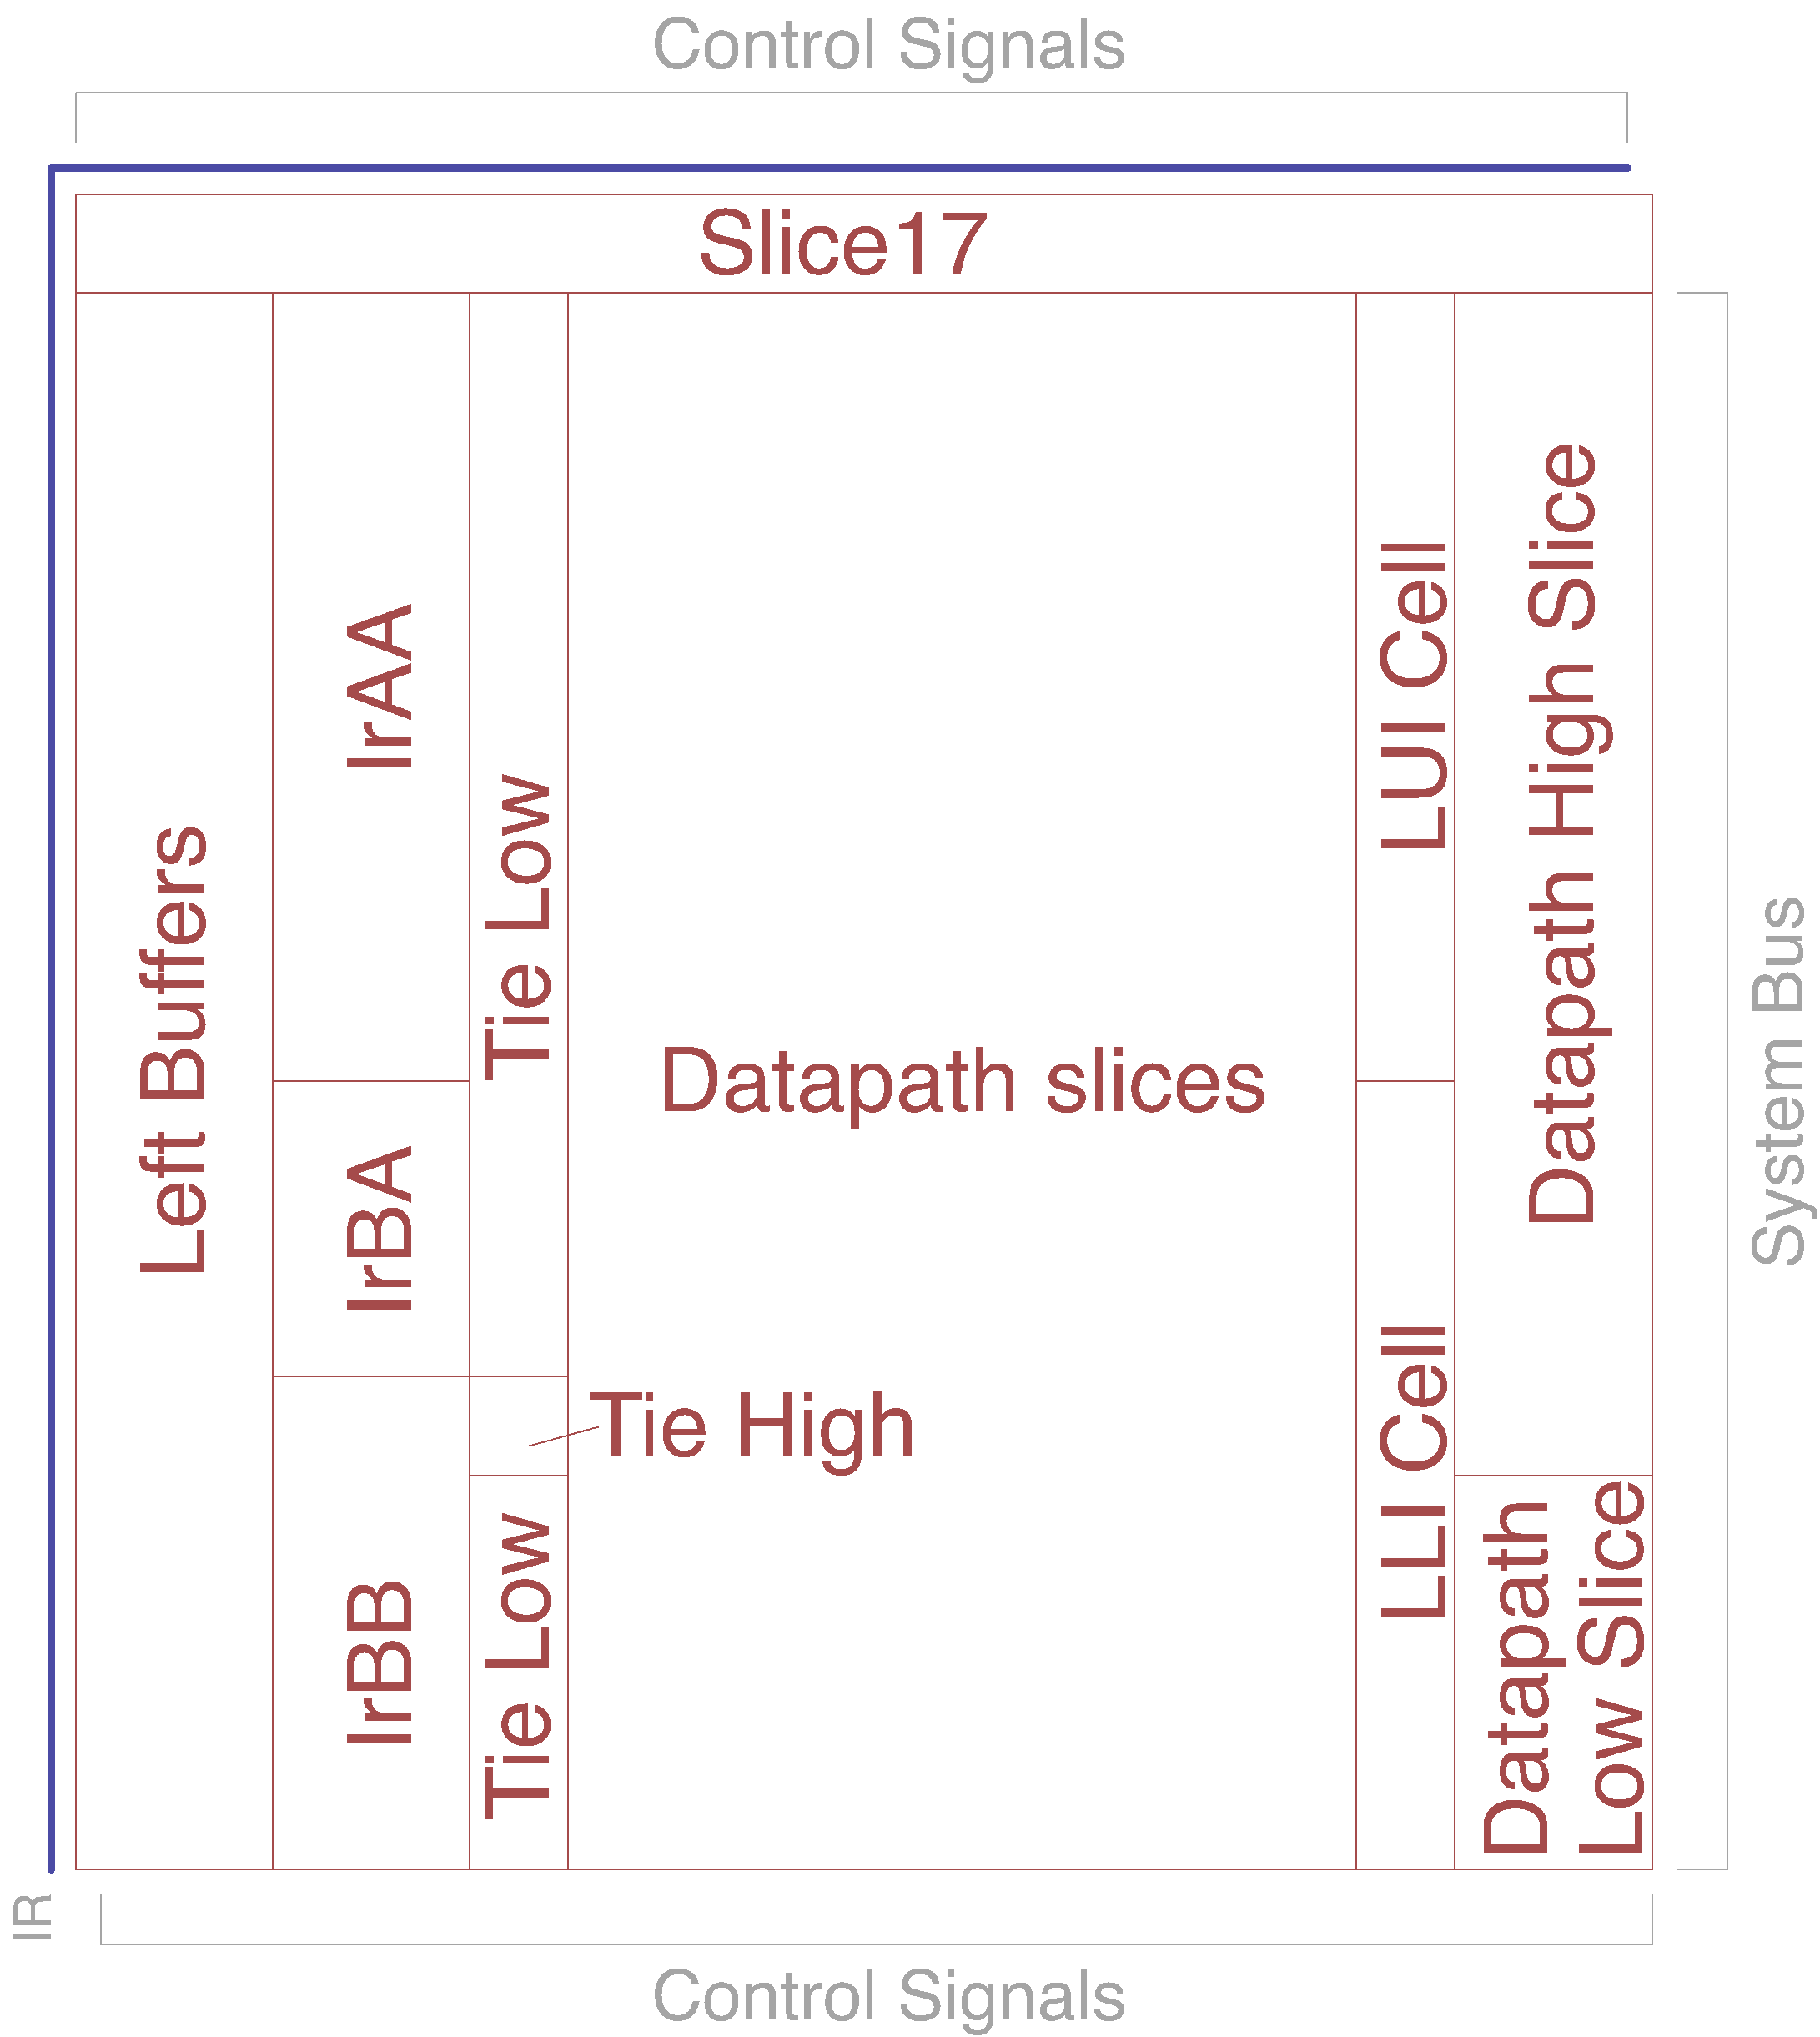
\includegraphics[width=\textwidth]{../../eagle/Datapath/datapath.png}
%\caption{Module layout to make the full datapath.}
%\label{fig:datapath:block}
%\end{figure}


\section{Controller}
\label{sec:controller}

The controller is a Mealy machine used to sequence operations performed on the datapath.
Figure~\ref{fig:ControlBlock} contains all inputs, outputs and internal registers.
There are $7$ labelled inputs including two $4$ bit buses and one $8$ bit bus.
There are $26$ labelled outputs including five $4$ bit buses and one $3$ bit bus.
Typedefs, defined in a global file, are used for some single bit outputs and all bus outputs to keep decoding consistent in control and the datapath. 


\begin{figure}[t]
   \centering
    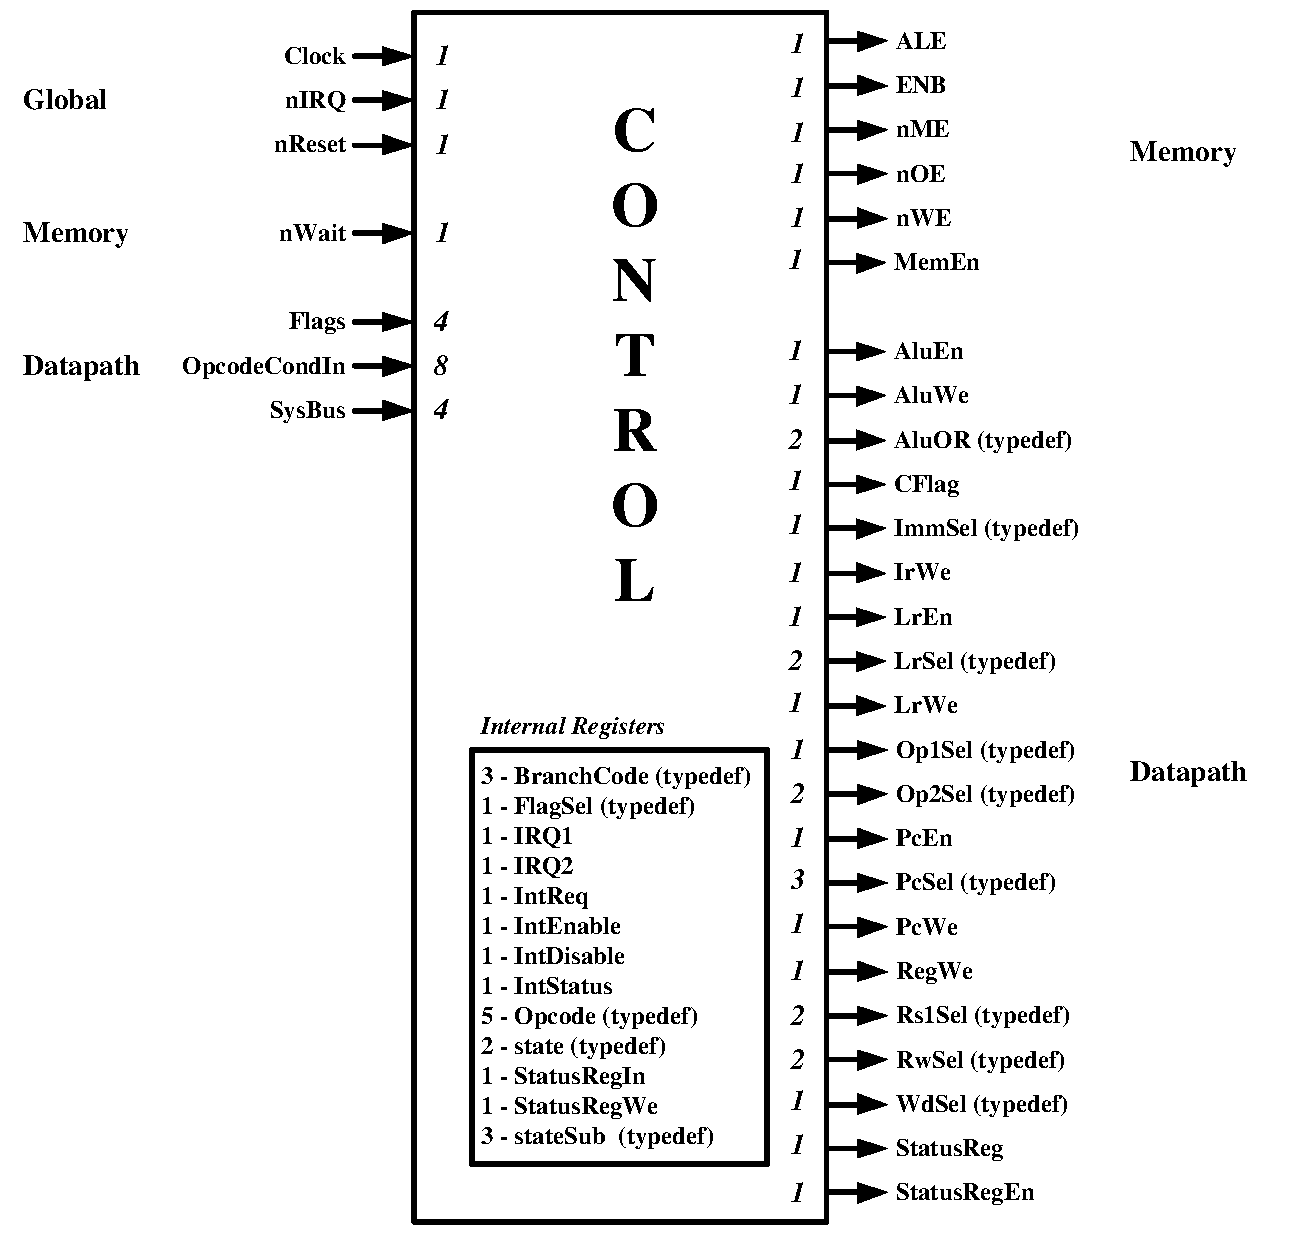
\includegraphics[width = 0.9\textwidth]{ControlPinout.pdf}
		\caption{Inputs, outputs and internal registers of the control block.}% \todo[inline]{Maybe change to IEEE symbols if we have time, AJR: we still have the eagle d-types but I think it would look a bit messy} }
   \label{fig:ControlBlock}
\end{figure}

Three main states exist to service the fetch, execute and interrupt stages.
Five sub states are used within the main states to further coordinate operation.
The ASM chart in figure~\ref{fig:MainStateASM} describes state changes using the sub state, opcode and interrupt request signal.   
Linked state machines are are used to produce the 
When \textit{nReset} is asserted the machine will return to the first cycle of the fetch state.
\todo[inline]{HSL: @AJR - this has an incomplete sentence in.}



\begin{figure}[ht]
   \centering
    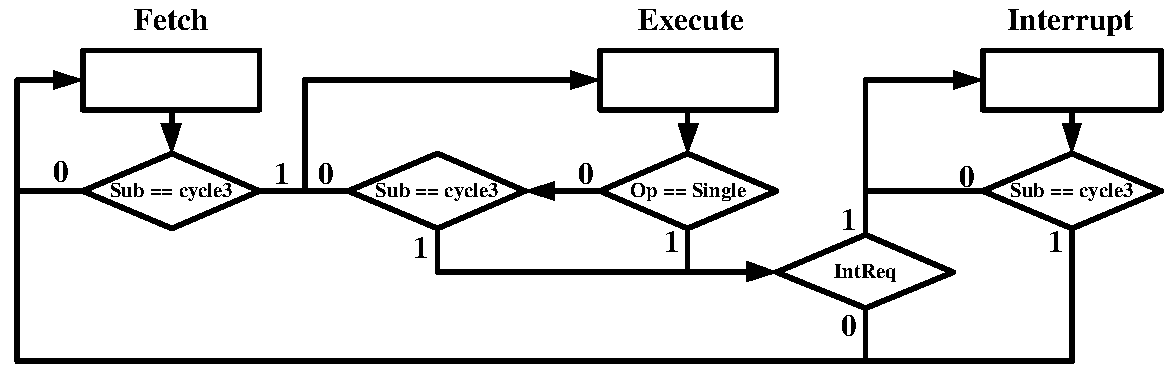
\includegraphics[width = \textwidth]{MainStateASM.pdf}
		\caption{ASM chart of controller main states.}
		\label{fig:MainStateASM}
\end{figure}








\subsection{Fetch}

Fetching an instruction from memory requires placing the program counter on the address bus then reading the instruction in to the instruction register. 
The state machine described in Figure~\ref{fig:FetchASM} asserts signals associated with memory access and delays if the slow memory access input, \textit{nWait}, is set.
When the transition from \textbf{cycle3} to \textbf{cycle0} is made the main state machine, Figure~\ref{fig:MainStateASM}, also make as transition therefore severing the link to this machine. 

\begin{figure}[ht]
   \centering
    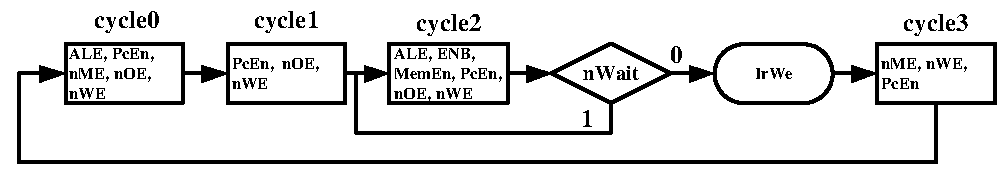
\includegraphics[width = \textwidth]{FetchASM.pdf}
		\caption{ASM chart of sub state transitions in the fetch stage.}
		\label{fig:FetchASM}
\end{figure}





\subsection{Execute}

The instruction fetched from memory is decoded in one cycle
This is a variable length stage that takes either $1$ or $4$ cycles depending on whether the instruction in the requires memory access.
After the instruction has been executed the \textit{IntReq} is used to 
\todo[inline]{HSL: @AJR - incomplete}

\begin{figure}[ht]
   \centering
    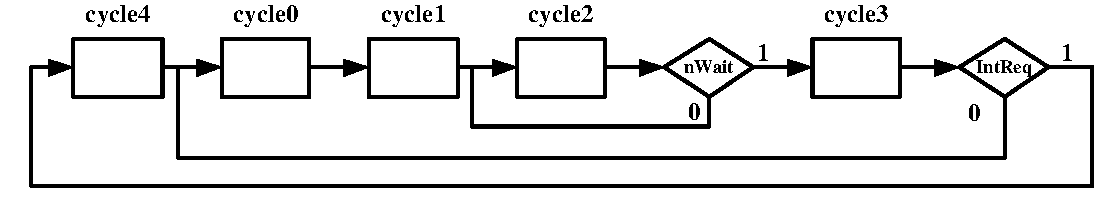
\includegraphics[width = \textwidth]{ExecuteASM.pdf}
		\caption{ASM chart of sub state transitions in the execute stage.}
		\label{fig:ExecuteASM}
\end{figure}





\subsection{Interrupt}

The circuit in Figure~\ref{fig:IntReqCircuit} is used to generate a interrupt request.
To avoid problems introduced by metastability the external \textit{nIRQ} signal is retimed using two D-types.
\textit{IntEnable} can only be set in code using the \textbf{ENAI} instruction.
\textit{IntDisable} is set when the processor is interrupted and also in code using the \textbf{DISI} instruction.
The end register contains \textit{IntStatus} which is low at reset therefore interrupts are off by default. 

\begin{figure}[ht]
   \centering
    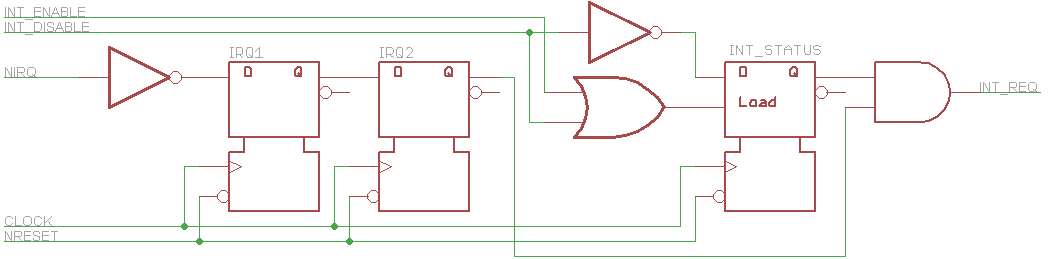
\includegraphics[width = \textwidth]{Interrupt.png}
		\caption{IntReq generation circuit.}
		\label{fig:IntReqCircuit}
\end{figure}


Entering an interrupt service routine (ISR) is completely handled in hardware. 
Interrupts are disabled and override functionality is used to decrement the stack pointer therefore allowing the program counter to be pushed to the stack.
The program counter is forced to address $0x0010$ which contains the code for ISR. 
The first operation in the ISR is \textbf{STF} which also places the flags, located in the control unit, on the stack.

When finished the second to last operation, \textbf{LDF}, loads the flags back in to the control unit.
This is similar to a \textbf{POP} operation but writes to the control unit instead of a general purpose register. 
The final operation is a \textbf{RETI} which again is similar but writes to the program counter.

A bidirectional data interface to the control unit is required to facilitate these operations. 
Figure~\ref{fig:FlagCircuit} contains the circuit used to load and store flags inside the control unit.
The $4$ bit word containing the flags is can be sourced from either the ALU or the bottom bits of SysBus. 
When storing the flags in memory the output of the status register must be placed on SysBus where the upper $12$ bits are all set to zero;  

\begin{figure}[ht]
   \centering
    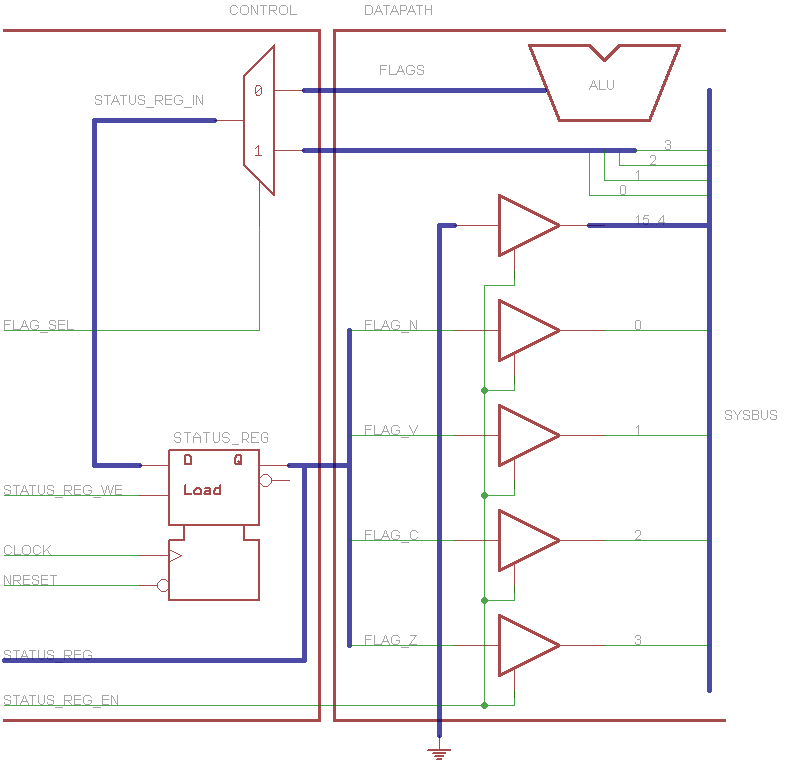
\includegraphics[width = 0.7\textwidth]{ControlIF.png}
		\caption{Control unit flag interface.}
		\label{fig:FlagCircuit}
\end{figure}





\subsection{Synthesis}

The controller was synthesised using Cadence Encounter. 
This provided a gate level netlist which was then used for place and route.
Both Magic and L-Edit place and route tools were used. 

The Magic place and route had a considerably larger routing channel than L-Edit the cells were all placed in one long row. 
This was suboptimal as it resulted in a lot of dead space within the floorplan.

The L-Edit place and route provided far better results. 
The datapath and controller were approximately the same width. 
The I/Os were able to be positioned around the module to reduce the overall wiring needed in the full floor plan. 
Most of the datapath control signals were routed to the top of the module to reduce the wiring channel needed between the cotroller and datapath.
All the memory access signals were routed to the left of the controller to make easier connections to the pad ring. 
The controller was also connected to the low nibble of the input data. 
This was connected at the bottom of the controller to reduce wiring needed. 
Finally, decoder signals and flag inputs were routed to the right of the control. 



%  CPU_Design.tex
%  Document created by seblovett on seblovett-Ubuntu
%  Date created: Thu 17 Apr 2014 15:14:45 BST
%  <+Last Edited: Thu 17 Apr 2014 15:36:00 BST by seblovett on seblovett-Ubuntu +>


\section{CPU}

%Overall layout 

The datapath and the control units were designed to allow them to connect together with as small a wiring channel as possible. 
All the I/Os were placed in each of the blocks to minimize the routing between the module and the pad ring. 
The pad ring used had a core size of $1505.00\mu m \times 1500.70\mu m$. 
The total size of the chip including the pad ring is $ 2150.00\mu m \times 2145.70\mu m$, a total area of $4.6mm^2$.

The controller was positioned below the datapath as it needed a connection to the lowest nibble of the system bus. 
The control signals between the datapath and controller were then placed to minimise the routing between them. 
This placement is at the expense of some control signals being routed to above the datapath. 

A net list was created and the magic autorouter was used.
This routed all the signals between the controller, datapath and the pad ring. 
The power lines were routed manually to the correct sizes. 

A large amount of polysilicon and the name of the processor, \textsc{Samurai}, is placed in the routing channels of the CPU to satisfy the design rule checks. 
A N-ohmic guard ring is also placed around the design and is connected to the core supply.
A large block of not\_pwell paint is used to explicitly define all undefined areas. 






%  Testing.tex
%  Document created by seblovett on seblovett-Ubuntu
%  Date created: Thu 17 Apr 2014 15:23:39 BST
%  <+Last Edited: Thu 17 Apr 2014 17:34:00 BST by seblovett on seblovett-Ubuntu +>


\chapter{Testing}

%  Register_Test.tex
%  <+Last Edited: Sun 11 May 2014 21:24:04 BST by seblovett on seblovett-Ubuntu +>

\section{Register Block}

%Include Sub tests - of slice and decoder (if app)
Tests were implemented for the decoder and bitslice modules implemented in Magic. 
A full module test was also written. 
The same test was designed to be run on both the Magic layout and the behavioural systemverilog design. 
This allowed the full operation of the behavioural model and implemented layout to be verified to the same standard. 

The bitslice test loads one bit of data into each register, and checks that it can be read back on each of the data read lines.
Assertions are used to automate the checking of the bit slice.

The decoder is verified by exercising all the possible inputs to each of the decoders.
The one hot encoding output is then checked to be as expected for the current input. %correct to the input.
This is repeated for each read decoder, and the write decoder is verified to only output correctly when the write enable signal is high. 

The full test uses a ``task'' code block to write to a register and read the data back.
The data is then verified to be correct on both read ports.
This process is repeated 100 times to exercise different data on all the registers. 
Assertions are used to give a final pass/fail result allowing quick verification of the module.
The tests ensure the read buffers and the writing to each register is fully functional.

%why it is done.

%How it verifies everything - why it is complete



%  PC_Test.tex
%  <+Last Edited: Thu 17 Apr 2014 15:35:14 BST by seblovett on seblovett-Ubuntu +>

\section{Program Counter}

Include Sub tests - of slice and decoder (if app)

Explain tests - what is done

why it is done.

How it verifies everything - why it is complete

Show simulation results


%  IR_Test.tex
%  <+Last Edited: Thu 08 May 2014 13:30:49 BST by seblovett on seblovett-Ubuntu +>

\section{Instruction Register}


Explain tests - what is done
The test for the instruction register is for the magic layout only.
This test is written to exercise the storing and reading of the instruction register, and the sign extension.

The test beings by resetting the module and checking the instruction register output is 0. 
The register is then loaded with 65535 and verifies the output matches this value.

The sign extension is then tested. 
This is done by loading a value which should be sign extended if it is a 5 bit immediate, but not if it is a 8 bit immediate. 
The two outputs are verified for each value of the \textit{ImmSel} signal. 
This is then repeated by using a value that would be extended if it is 8 bit, but not if it is 5 bit. 

This verifies the operation of the instruction register and that the sign extension correctly functions. 
All behaviour is verified using assertions and giving a final pass/fail statement. 
This allowed for modifications to be easily verified. 


%  ALU_Test.tex
%  <+Last Edited: Mon 12 May 2014 09:52:22 BST by seblovett on seblovett-Ubuntu +>

\section{Arithmetic Logic Unit}
To promote the use of hierarchy within design the ALU is broken down into a number of sub-modules. 
These have been tested individually to ensure they operate as expected. 
Then they are combined into 16 bits without decoder for testing the combination of ALU and LLI slices. 
Since the LLI slices are either a single multiplexor or wires they will not be tested individually. 
They will form a part of the ALU Block testing. 
%All test results are shown in Appendix~\ref{chap:ALUTestResults}.

\subsection{ALU Slice}
Testing of this module was broken down into the different ALU functions to be performed: arithmetic, logic and shifting. 
Control inputs which effect the behaviour of arithmetic operations are \textit{SUB} and \textit{ZeroA}. 
As such tests were run to cover every combination of \textit{A}, \textit{B} and \textit{CIn} for addition and subtraction. 
Then \textit{ZeroA} was activated during each combination of \textit{B} and \textit{CIn}, while \textit{A} is held high, to ensure correct tying low of one input. 
%The test results are shown in Figure~\ref{fig:ALUSliceRes}. 
For subtraction tests, because additional logic for handling subtraction carrys is within the decoder, testing needed to account for both the carry in and borrow signals being the inverse of expected operation.
Logic operations are tested by using every input combination possible and comparing to the relevant logic table expected.
%The output of these tests are shown in Figure~\ref{fig:ALUSliceRes}. 
Testing of the shifting capabilities was done by setting all inter-slice inputs high with the input \textit{A} held low. Then for each case of: left, right and left with \textit{B} input shifting, different immediate signals were set to observe the propagation of bits through the slice. 
If a bit in the 4 bit immediate is high, a 1 would be outputted in the next adjacent bit of the output. 
This is \textit{OutLeft} for left shifting or \textit{OutRight} for right shifting.
% as shown in Figure~\ref{fig:ALUSliceRes}.
Although shifting operation was as expected, much clearer testing will be done during 16 bit block tests to emulate typical running. 

\subsection{ALU Decoder}
The main testing of the ALU decoder module requires ensuring a correct response to each possible Opcode. 
This was done by cycling through in-putted Opcode values, with assertion checking using an always statement which activates every time an input changes. 
These check against the logic equations for each output signal given in Equations~\ref{eq:DecBasicS}~to~\ref{eq:DecBasicF}. As well as Table~\ref{tab:contrOuts} for single Opcode signals. 
Signals \textit{UseC} and {\textit{ShSign} are still checked for correspondence with this table, even though they are not outputs from the decoder module. 

Flag testing sets the Opcode to either \textbf{ADC} or \textbf{SUC} and checks each combination of relevant inputs to ensure V, C and  are as expected. N remains untested as there is no logic to test. 
Shift operations set the 4 bit immediate to a range of values which cover each output Sh8-Sh1 being activated at least once. A full test from 0 to 15 is not needed. The input bit for arithmetic shifting is also tested by enabling/disabling ASign. 

\subsection{ALU Block}
Testing of 16 connected slices took a similar approach to an individual slice, but with full 16 bit values. 
Arithmetic used two arbitrary input values combined with each possible carry in value, accounting for both addition and subtraction operation. 
Logic tests ensure each bit pair is operated upon independently of the rest by using an arbitrary string of bits. 
Whilst shift tests run through both directions and a number of shifting amounts, similar to slice testing, to show the selected input is shifted by the expected number of bits. 
Then the \textbf{LUI} instruction was tested separately to ensure successful 8 bit left shifting operation. 
Finally \textbf{LLI} was tested using the same values as in previous tests, to check upper and lower byte concatenation of inputs A and B respectively. 

%  Datapath_Test.tex
%  <+Last Edited: Thu 17 Apr 2014 15:35:51 BST by seblovett on seblovett-Ubuntu +>

\section{Datapath}
\review{Datapath Test}
%\todo[color=cyan, inline]{Include Sub tests - of slice and decoder (if app)}
%\todo[color=cyan, inline]{Explain tests - what is done}
%\todo[color=cyan, inline]{why it is done.}
%\todo[color=cyan, inline]{How it verifies everything - why it is complete}
%\todo[color=cyan, inline]{Show simulation results}
\todo[inline]{Fix slice testing problems}
\todo[inline]{Main - Change testing values to ensure changes to output}
\todo[inline]{(Operand Selection)}

Testing of the complete datapath was done at both the slice level and fully assembled. These modules are highly hierarchical and as such each sub-module would have been tested during the implementation of it. Since the datapath slice is simply an accumulation of sub-modules and some multiplexors, only the top-level circuitry needs to be tested. This was made up of input selection multiplexors for regBlock and the ALU. The first was tested by changing the inputs AluOut and SysBus and switching between them, asserting if the output is correct. A similar approach was taken for the remaining logic.

Prior to testing it was necessary to reset register values, which was done by extending Clock and nReset signals to the edge of the cell as testing inputs. This does break hierarchy rules within magic, but prevents the need for a slightly larger cell to access global signals. 

The assembled datapath was tested by checking the flow of data between each node on the diagram shown in Figure~\ref{fig:architecture}, with additional multiplexed nodes between the IR and register address select signals; Rs1, Rs2 and Rw. Each of these nodes is an array of internal signals either from each slice or as outputted from the decoders in slice 17. Then these nodes are grouped in accordance with their location in the datapath and tested separately. These groupings were: multiplexors from IR, Operand Selection, ALU output, link register connections, program counter connections, writing general purpose registers, ALU override and status register. As with slice testing, every operation performed by the ALU or GPRs were not tested as they would have been for the individual module testing. 
%  Control_Test.tex
%  <+Last Edited: Thu 17 Apr 2014 15:36:24 BST by seblovett on seblovett-Ubuntu +>

\section{Controller}

Activity in the control unit is dependent on the upper byte of data in the instruction register which is broken down into the $5$ but opcode and the $3$ bit branchcode.  
The instruction register is populated in the fetch stage, which is always the same, so a function \textbf{DoFetch} is used to update the instruction register with different value for testing.
At this point an umbrella test is used to verify no output of the controller is ever unknown during any state.

After each fetch the variable length execute stage is tested.


\todo[inline]{Add listing package, need better machine to test}
\lstinputlisting[style=C,label=lst:ControlVector.c,caption=Control unit test vector.]{Code/ControlVector.c}


Include Sub tests - of slice and decoder (if app)

Explain tests - what is done

why it is done.

How it verifies everything - why it is complete

Show simulation results


%  CPU_Test.tex
%  <+Last Edited: Sun 11 May 2014 09:50:12 BST by seblovett on seblovett-Ubuntu +>

\section{CPU}

A full system test was devised. 
This consisted of filling the program memory with random data. 
Two simulations are then run: one with the behavioural model and one on the extracted netlist. 
If the two models are identical, then the contents of the memory and the registers should match at the end of the simulations.

A few issues were encountered in the implementation of the test.
Firstly, memory operations caused issues. 
As the memory map contains undefined areas, load operations could possilby load invalid memory into the design.
Due to the Von Neuman architecture, this invalid memory could be stored back to the program memory and cause the processor to crash. 
Invalid memory cannot be verified, resulting in the test failing. 
For this reason, all memory operations were removed from the memory.
Similarly, jumps were removed also removed to prevent the program jumping to an invalid memory location. 

Interrupt intstructions were also removed due to the memory returning issue with RETI, STF, LDF, and the lack of verification for the enable and disable interrupt instructions. 
Finally, due to the unpredicatable nature for some flags after logic operations, any arithmetic instructions with flag depencies (ADCI, ADCIB etc.) are also removed. 
The removed operations are replaced with ADDIB R0 127 to save repeatedly checking the data. 

%Verilog was implemented to stop the simulation when the program counter reach $0x7FF$. 
%The contents of the 8 general purpose registers were then saved to a file. 
The code implemented in Verilog to save the registers is shown in Listing~\ref{lst:wn:verilog}.
The Program Counter is probed depending on which simulation is been run.
On each clock, it is checked.
If the Program Counter is greater than or equal to $0x07FF$ (the end of valid memory), the simulation is terminated.
The values of the registers are saved to a file. 
%\todo[inline]{Include verilog listing?}

A python script was written and does the following:
\begin{enumerate}
\item Generate 2048 words of random data
\item Remove any invalid instructions (as described above)
\item Write operations to a hex file
\item Run Behavioural simulation
\item Run Extracted simulation
\item Compare the saved files
\end{enumerate}

The comparison checks the final register values and indicate a pass or fail. 
A pass is issued if all registers match. 
The test on the processor showed that there is an inconsistency between the two processors. 
The output of the test is shown in Listing~\ref{lst:wn:output}.
However, due to the use of random data, this is not a repeatable test and is difficult to debug the issues. 

\todo[inline,color=red]{BUG: When I include the definitions.tex and change the style of the verilog listing, some contention happens with the xcolor package and breaks things.}
\lstinputlisting[firstline=184,label=lst:wn:verilog,caption=Whitenoise test verilog]{../../Design/Implementation/verilog/behavioural/monitor.sv}



\begin{lstlisting}[label=lst:wn:output,caption={Output of the white noise test}]
Reg	B	E	P/F
---------------------------
0	007f	007f	P
1	5504	0073	F
2	faff	faff	P
3	581a	581a	P
4	aafc	aafc	P
5	04d4	04d4	P
6	7cff	0001	F
7	faf4	faf4	P
White Noise Test Failed.
\end{lstlisting}

%\todo[inline]{include a shot of the test results}


%  Conclusion.tex
%  Document created by seblovett on seblovett-Ubuntu
%  Date created: Thu 17 Apr 2014 15:25:42 BST
%  <+Last Edited: Sun 11 May 2014 10:55:58 BST by seblovett on seblovett-Ubuntu +>


\chapter{Conclusion}
%\incomplete{Conclusion}
\review{Conclusion}
\todo[inline, color=green]{MW:Ive expanded alot on what was here for more overview status of system and some evaluative conclusions}

The processor designed is a 16 bit RISC architecture which has a fully completed layout and is design rule checked. 
With added novel functionality including; multi-bit shifting, stack-specific operation \texttt{PUSH} and \texttt{POP}, varied length immediate value support and 8 GPRs with dedicated link register and program counter. 
Each module has been individually tested and verified.
However, there is a discrepancy between the behavioural model and the extracted layout.
In the individual modular test sequences, this discrepancy was not noticed. 
It is not known if the bug exists in the layout or the behavioural model. 

Appendix~\ref{ch:pm} discusses the workings of the group and the project management.
This is rounded off with individual reflections from group members.
Appendix~\ref{ch:dol} shows the overall Division of Labour within the group for the entire project.

Given the size of the group, the level of functionality gained and the progress made is higher than the original expectations of the group. 
However this has lead to a less optimized design due to the limited manpower available. 
As with interrupt support being an additional aspect not forming a part of the initial design. 
It also became apparent from the ``Balloon Debate'' that our design focussed more advanced functionality than operating speed and physical size which should have had greater consideration. 

Overall, the project has been successful in producing a functional general purpose microprocessor.  
Whilst supporting material such as a symbolic assembler has been produced to a good standard to aid any programmer with using this system. 
\appendix

\chapter{Instruction Set Summary}
\label{chap:AppISS}

\begin{table}[t]
\centering
\footnotesize
\renewcommand{\arraystretch}{1.2}
\makebox[\linewidth]{
\begin{tabular}{r|c|c|c|c|c|c|c|}
	\multicolumn{1}{c}{} & \multicolumn{1}{c}{\bf Mnemonic} & \multicolumn{1}{c}{\bf Syntax} & \multicolumn{1}{c}{\bf Semantics} & \multicolumn{1}{c}{\bf Flags} & \multicolumn{1}{c}{\bf Encoding} & \multicolumn{1}{c}{\bf Opcode} & \multicolumn{1}{c}{\bf Cond.} \\
	\cline{2-8}
	1 & ADD   & ADD Rd, Ra, Rb      & Rd $\leftarrow$ Ra + Rb       & c,v,n,z & A & 00010 & - \\
	2 & ADDI  & ADDI Rd, Ra, \#imm5 & Rd $\leftarrow$ Ra + imm5 	& c,v,n,z & A & 00110 & - \\
	3 & ADDIB & ADDIB Rd, \#imm8    & Rd $\leftarrow$ Rd + imm8     & c,v,n,z & B & 00011 & - \\
	4 & ADC   & ADC Rd, Ra, Rb      & Rd $\leftarrow$ Ra + Rb + c   & c,v,n,z & A & 00100 & - \\
	5 & ADCI  & ADCI Rd, Ra, \#imm5 & Rd $\leftarrow$ Ra + imm5 + c & c,v,n,z & A & 00101 & - \\
	6 & NEG   & NEG Rd, Ra          & Rd $\leftarrow$ 0 - Ra        & c,v,n,z & A & 11010 & - \\
	7 & SUB   & SUB Rd, Ra, Rb      & Rd $\leftarrow$ Ra - Rb       & c,v,n,z & A & 01010 & - \\
	8 & SUBI  & SUBI Rd, Ra, \#imm5 & Rd $\leftarrow$ Ra - imm5     & c,v,n,z & A & 01110 & - \\
	9 & SUBIB & SUBIB Rd, \#imm8    & Rd $\leftarrow$ Rd - imm8     & c,v,n,z & B & 01011 & - \\
	10& SUC   & SUC Rd, Ra, Rb      & Rd $\leftarrow$ Ra - Rb - c   & c,v,n,z & A & 01100 & - \\
	11& SUCI  & SUCI Rd, Ra, \#imm5 & Rd $\leftarrow$ Ra - imm5 - c & c,v,n,z & A & 01101 & - \\
	12& CMP   & CMP Ra, Rb          & Rd $\leftarrow$ Ra - Rb       & c,v,n,z & A & 00111 & - \\
	13& CMPI  & CMPI Ra, \#imm5     & Rd $\leftarrow$ Ra - imm5     & c,v,n,z & A & 01111 & - \\
	14& AND   & AND Rd, Ra, Rb      & Rd $\leftarrow$ Ra \texttt{AND} Rb     & n,z     & A & 10000 & - \\
	15& OR    & OR Rd, Ra, Rb       & Rd $\leftarrow$ Ra \texttt{OR} Rb      & n,z     & A & 10001 & - \\
	16& XOR   & XOR Rd, Ra, Rb      & Rd $\leftarrow$ Ra \texttt{XOR} Rb     & n,z     & A & 10011 & - \\
	17& NOT   & NOT Rd, Ra          & Rd $\leftarrow$ \texttt{NOT} Ra        & n,z     & A & 10010 & - \\
	18& NAND  & NAND Rd, Ra, Rb     & Rd $\leftarrow$ Ra \texttt{NAND} Rb    & n,z     & A & 10110 & - \\
	19& NOR   & NOR Rd, Ra, Rb      & Rd $\leftarrow$ Ra \texttt{NOR} Rb     & n,z     & A & 10111 & - \\
	20& LSL   & LSL Rd, Ra, \#imm4  & Rd $\leftarrow$ Ra $<<$ imm4  & n,z     & A & 11111 & - \\
	21& LSR   & LSR Rd, Ra, \#imm4  & Rd $\leftarrow$ Ra $>>$ imm4  & n,z     & A & 11101 & - \\
	22& ASR   & ASR Rd, Ra, \#imm4  & Rd $\leftarrow$ Ra $>>>$ imm4 & n,z     & A & 11100 & - \\
	23& LDW   & LDW Rd, [Ra, \#imm5]& Rd $\leftarrow$ Mem[Ra + imm5]& -       & C & 00000 & - \\
	24& STW   & STW Rd, [Ra, \#imm5]& Mem[Ra + imm5] $\leftarrow$ Rd& -       & C & 01000 & - \\
	25& LUI   & LUI Rd, \#imm8      & Rd $\leftarrow$ {imm8, 0}     & -       & B & 10100 & - \\
	26& LLI   & LLI Rd, \#imm8      & Rd $\leftarrow$ {Rd[15:8], imm8}& -     & B & 10101 & - \\
	27& BR    & BR LABEL            & PC $\leftarrow$ PC + imm8     & -       & D & - & 000 \\
	28& BNE   & BNE LABEL           & (z==0)?PC $\leftarrow$ PC + imm8& -     & D & - & 110 \\
	29& BE    & BE LABEL            & (z==1)?PC $\leftarrow$ PC + imm8& -     & D & - & 111 \\
	30& BLT   & BLT LABEL           & (n\&$\sim$v \texttt{OR} $\sim$n\&v)?PC $\leftarrow$ PC + imm8& - & D & - & 100 \\
	31& BGE   & BGE LABEL           & (n\&v \texttt{OR} $\sim$n\&$\sim$v)?PC $\leftarrow$ PC + imm8& - & D & - & 101 \\
	32& BWL   & BWL LABEL           & LR $\leftarrow$ PC + 1; PC $\leftarrow$ PC + imm8& - & D & - & 011 \\
	33& RET   & RET                 & PC $\leftarrow$ LR            & -       & D & -     & 010 \\
	34& JMP   & JMP Ra, \#imm5      & PC $\leftarrow$ Ra + imm5     & -       & D & -     & 001 \\
	\multirow{2}{*}{35}& \multirow{2}{*}{PUSH}  & PUSH Ra             & R7 $\leftarrow$ R7 - 1; Mem[R7] $\leftarrow$ Ra; & \multirow{2}{*}{-} & \multirow{2}{*}{E} & \multirow{2}{*}{-} & \multirow{2}{*}{-} \\
	  &       & PUSH LR             & R7 $\leftarrow$ R7 - 1; Mem[R7] $\leftarrow$ RL; &   &   &   &   \\
	\multirow{2}{*}{36}& \multirow{2}{*}{POP}   & POP Ra              & Mem[R7] $\leftarrow$ Ra; R7 $\leftarrow$ R7 + 1; & \multirow{2}{*}{-} & \multirow{2}{*}{E} & \multirow{2}{*}{-} & \multirow{2}{*}{-} \\
	  &       & POP LR              & Mem[R7] $\leftarrow$ RL; R7 $\leftarrow$ R7 + 1; &   &   &   &   \\
	37& RETI  & RETI                & PC $\leftarrow$ Mem[R7]       & -       & F & -     & 000 \\
	38& ENAI  & ENAI                & IntEnFlag $\leftarrow$ 1      & -       & F & -     & 001 \\
	39& DISI  & DISI                & IntEnFlag $\leftarrow$ 0      & -       & F & -     & 010 \\
	40& STF   & STF                 & R7 $\leftarrow$ R7 - 1; Mem[R7] $\leftarrow$ Flags; & - & F & - & 011 \\
	41& LDF   & LDF                 & Flags $\leftarrow$ Mem[R7]; R7 $\leftarrow$ R7 + 1; & c,v,n,z & F & - & 100 \\
	\cline{2-8}
\end{tabular}
}
\end{table}
%\chapter{Test Results}

\section{ALU Results}
\label{chap:ALUTestResults}

\begin{figure}[h]
	\centering
	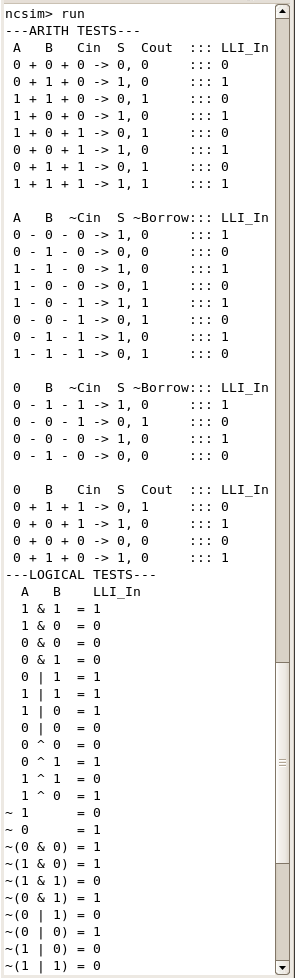
\includegraphics[scale=0.72]{results/ALUSliceA.png}
	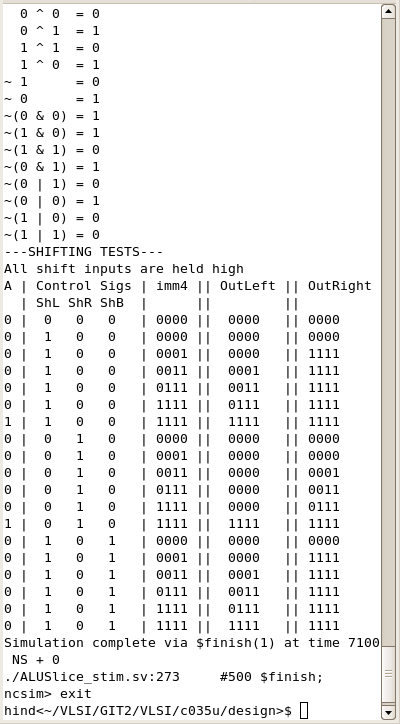
\includegraphics[scale=0.72]{results/ALUSliceB.png}
	\caption{Test Results for ALUSlice}
	\label{fig:ALUSliceRes}
\end{figure}
\begin{figure}[h]
	\centering
	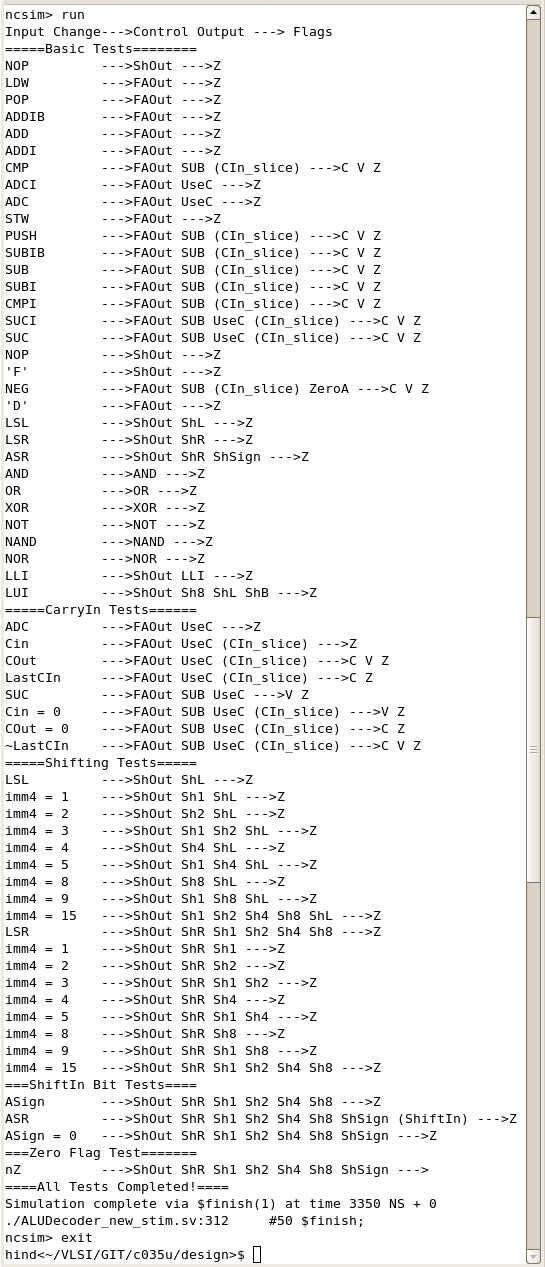
\includegraphics[scale=0.56]{results/ALUDecoder.png}
	\caption{Test Results for ALUDecoder}
	\label{fig:ALUDecoderRes}
\end{figure}
\begin{figure}[h]
	\centering
	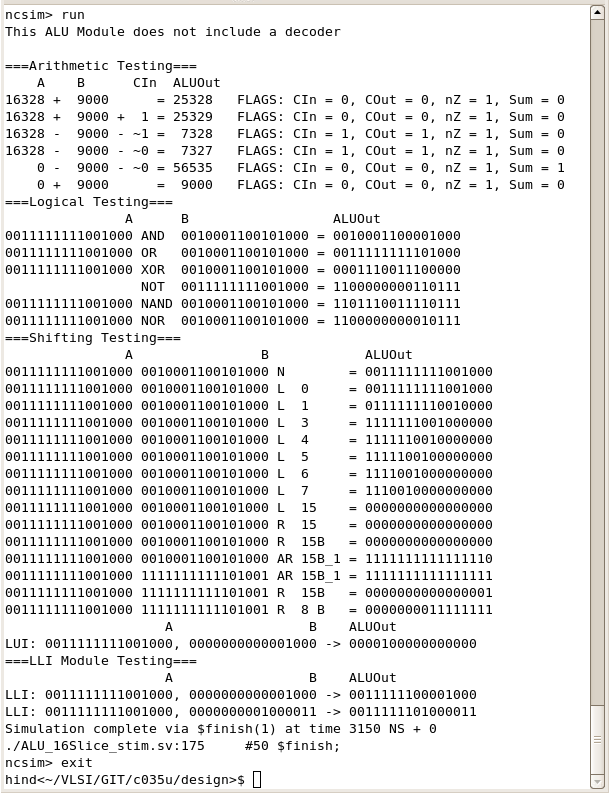
\includegraphics[scale=0.72]{results/ALUBlock.png}
	\caption{Test Results for 16 Slice Block}
	\label{fig:ALUBlockRes}
\end{figure}

%  ProjectManagement.tex
%  Document created by seblovett on seblovett-Ubuntu
%  Date created: Thu 17 Apr 2014 15:26:37 BST
%  <+Last Edited: Mon 12 May 2014 16:32:25 BST by seblovett on seblovett-Ubuntu +>

\chapter{Project Management}\label{ch:pm}
%\incomplete{Project Management}


Groups members are referred to by initials in this Chapter as follows:
\begin{enumerate}
\item HL - Henry Lovett (hl13g10)
\item MW - Martin Wearn (mw20g10)
\item AJR - Ashley Robinson (ajr2g10)
\item ARR - Anusha Reddy (arr1g13)
\end{enumerate}

\section{Group formation}

The group initially contained five students. 
At the start of the project, two of the original students left the group: one joined another team, and one dropped the module.
This left the group with three members - AJR, MW and HL. 
Discussions were then undertaken as to if the group wanted / needed a fourth member. 
As the group could not come to a unanimous decision, one for a fourth member, one against and one who was happy either way, Iain's advice for having a fourth member was taken. 

The original member of the group did not wish to rejoin the group.
Instead, a colleague of the original member was offered to join.
%This formed the group members. 

In the first discussions with the group, HL was appointed as group leader. 

\section{Meetings}

The group held two meetings per week at scheduled times: Monday afternoons at 15:00 and Thursday afternoons at the end of the lab.
%A meeting was always held towards the end of the Thursday lab session.
All meetings were chaired by HL.

Agendas for Monday meetings were sent out by HL, usually 24 hours beforehand. 
The Monday meeting was there to discuss any work done since Thursday or outstanding issues. 
The other task for the Monday meeting was to confirm the milestones for the week.
This ensured that all group members were aware of who was responsible for what that week to avoid confusion that could potentially cause a delay in a hand-in.
Ongoing tasks were discussed at these meetings also.
Work for the lab on Thursday was allocated so members were able to commence work without hindrance.

The meeting at the end of the Thursday lab was to discuss the progress made that day. 
As this was the main working time, smaller aspects were discussed during the day between individual members.
The meeting at the end of the lab allowed everyone to know any design changes or issues encountered and the problems discussed.
Work for the time outside of the lab was then allocated at this point.


\section{Skills Assessment}

A small skills audit was done in the first meeting. 
The results of this are seen in Table~\ref{tab:pm:skills}.
It was apparent early on that ARR was not comfortable with a lot of the skills required.
Realising this early in the project allowed the work to be allocated optimally throughout the group members, particularly ensuring ARR was given realistic objectives and adequate help where required.

\begin{table}[h]
\centering
\caption{Skills Audit for Team R4. A 5 means very competent, 1 is not competent.}
\label{tab:pm:skills}
\begin{tabular}{l*{4}{p{1cm}}}\hline
Task 			& HL & MW & AJR & ARR \\ \hline
Verilog 		& 4  & 4  & 4   & 2   \\
Magic Layout		& 4  & 4  & 3   & 4   \\
Assembly Language	& 3  & 3  & 3   & 1   \\
Processor Design	& 4  & 4  & 4   & 1   \\ 
Git			& 4  & 3  & 4   & 1   \\ \hline
\end{tabular}
\end{table}


\section{Work Breakdown}

The skills audit provided the basis for the initial work allocations.
Preferences were given and the group was roughly broken into two sections: HL and AJR were to pursue the SystemVerilog development, MW and ARR would do the Magic layout.
Although the work was distributed this way, it was by no means a comprehensive divide.
ARR and MW were to also write SystemVerilog testbenches, and HL and AJR would be responsible for the synthesis and layout of the control unit.
The initial breakdown was done to give the team a starting point.

%The milestone responsibilities were also allocated, loosely based on the skills audit.


\section{Git}
%Git was used for revision control and branching (interrupt development)

HL, MW and AJR all had worked together previously, therefore the use of Git revision control was decided before the group was formed. 
When ARR joined the group, our file control was discussed, and alternative options were discussed. 
One idea from ARR was to use DropBox. 
This was a simple to use system, but would cause issues when multiple people worked on the same files. 
There was also no log of changes and broken files could have accidentally been integrated. 
The full recursive revision control with Git helped as if and when a file was committed that didn't work, it could be reverted to the previous version.
Change logs are also used with Git, allowing to see which files have changed, by who and why. 


The advantage to using Git was that the work could be branched.
This was exceptionally useful as the group was looking to implement interrupts.
The interrupt work could be done concurrently, but separately, to the normal work flow. 
If the group hadn't achieved the milestones for the interrupt development, no time would have been needed removing it.
At the point of success with interrupts, the work done was easily merged into the master branch. 

All group members agreed on the use of Git. 
HL and MW both spent time with ARR to help her understand the basics to be able to use Git.


\section{Github}
%Issue Tracking and task allocation using GitHub
Github is an online resource for hosting Git repositories. 
As well as the hosting, Github provides an issue tracking facility.
Issues were opened for items of work to be done, or for bugs found in the design.
The issue webpages provided a comment thread for the group members for discussion.

Issue tracking meant it was easy to keep an eye on what tasks were on going, complete or if it needed more time and resources to complete on time.
Issues can be allocated to group members, so the same task is not completed by multiple people. 
Github was extremely useful for this tracking and provided a common communication network for the group. 

\subsection{Git Additions by Group Member}

Github has the ability to extract statistics of the repository. 
This includes the commits, additions and deletions over time by each user (excluding merges). 
The number of commits is not an accurate method of measuring activity as different people have different commit habits.
For example, one member may commit a lot, but make little changes in each commit, whereas someone else may make a lot of changes, test and then commit.
Deletions are also included in the statistics, but are not a reliable measure as HL was responsible for keeping the repo clean and removing the temporary or unused files. 

However, the total additions is a more accurate measure. 
Magic files can be included in this measure as these are plain text files.
Report writing was done using \LaTeX, which in essence, is code and therefore the additions measure applies here too.

Due to ARR being introduced to Git, it would be expected that in the initial phase of the project, her commit count would be low, resulting in low additions also. 
Ideally, this would then increase to a reasonable level during the project. 
Some commits were done on behalf of ARR by HL in the early stages also, but this was not common.

Figure~\ref{fig:additions} shows the addition history in the repository. 
It is clear to see that HL employs a commit little and often style, where as MW and AJR commit more in less commits. 
The initial peak with AJR was the addition of an emulator he found.
If this is not taken into account, the total additions of HL, AJR and MW are approximately equal.  
It was expected that the additions of ARR would be lower than other members due to the learning curve needed for Git.
However, it is clear to see the 6,225 additions from ARR is significantly less than the rest of the group.

\begin{figure}
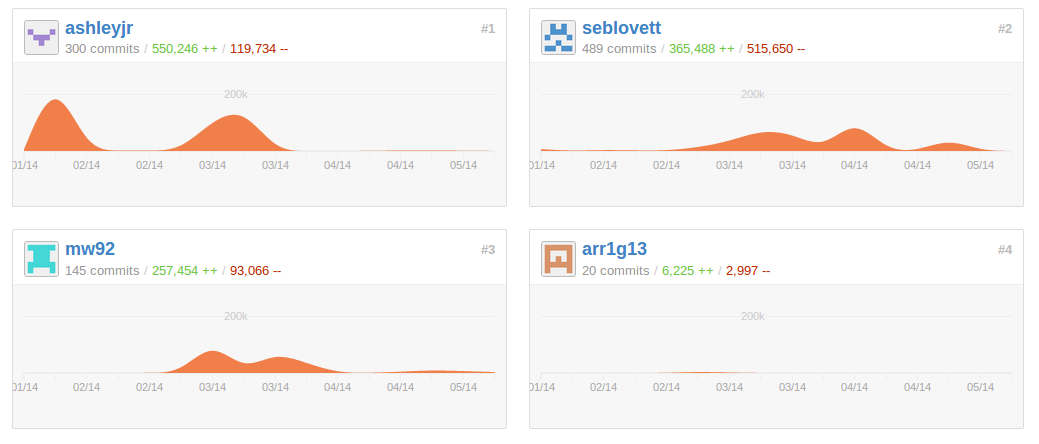
\includegraphics[width=\textwidth]{Figures/gitadditions.png}
\caption{Graph from Github showing the additions over time for each user. Additions are measured in lines in a file and shown in green. Deletions are shown in red. (seblovett = HL; ashleyjr = AJR; mw92 = MW; arr1g13 = ARR)}
\label{fig:additions}
\end{figure}


\section{Reflections}

This section contains individual reflections from group members. 
These are written to give everyone a chance to discuss their view of the group operation. 
ARR's reflection is not included. 
She was advised to include her own reflections in her individual report and given the same suggestions as to what it should include.

\subsection{HL}
\input{HL_Reflection.txt}
\subsection{MW}
\input{MW_Reflection.txt}
\subsection{AJR}
\input{AJR_Reflection.txt}
%\subsection{ARR}


%  DivisionOfLabour 
%  Document created by seblovett on seblovett-Ubuntu
%  Date created: Thu 17 Apr 2014 15:27:14 BST
%  <+Last Edited: Mon 05 May 2014 12:46:12 BST by seblovett on seblovett-Ubuntu +>


\chapter{Division of Labour}


\begin{table}[!h]
\begin{tabular}{p{0.8cm}p{\textwidth-10.2cm}p{1.7cm}p{1.7cm}p{1.7cm}p{1.7cm}}
     & Task             & \multicolumn{4}{c}{Percentage Effort on task} \\ \hline
     &  \textit{ECSID:}					& hl13g10 & ajr2g10 & mw20g10 & arr1g13 \\ \hline
1    & Initial Design					& 25	& 25	& 25 	& 25 \\ \hline 
2    & Verilog Behavioural Model			& 50	& 50	& 0 	& 0 \\ \hline 
2.1  & Interrupts 					& 40	& 40 	& 20 	& 0 \\ 
3    & Multiply Program					& 0	& 100	& 0 	& 0 \\ \hline 
4    & Magic Datapath					& 20	& 0	& 60 	& 20 \\ 
%4.1  & Registers					& 0	& 0	& 0 	& 0 \\  
%4.2  & Program Counter					& 0	& 0	& 0 	& 0 \\  
%4.3  & Instruction Register				& 0	& 0	& 0 	& 0 \\  
%4.4  & ALU						& 0	& 0	& 0 	& 0 \\ \hline 
5    & Verilog Cross Simulation				& 50	& 50	& 0 	& 0 \\ \hline 
6    & Control Unit Synthesis				& 100	& 0	& 0 	& 0 \\ \hline 
7    & L-Edit Control Unit				& 100	& 0	& 0 	& 0 \\ \hline 
8    & Final Floorplanning, Placement and Routing	& 100	& 0	& 0 	& 0 \\ \hline 
9    & Factorial Program				& 0	& 100	& 0 	& 0 \\ \hline 
10   & Random Program					& 0	& 100	& 0 	& 0 \\ \hline 
11   & Interrupt Program				& 0	& 100	& 0 	& 0 \\ \hline 
11   & Verilog Final Simulations and Cadence DRC	& 99	& 0	& 1 	& 0 \\ \hline 
12   & Assembler					& 2.5	& 2.5	& 95 	& 0 \\ \hline 
13   & Programmer's Guide Documentation			& 30	& 20	& 40 	& 10 \\ \hline 
%13.1  & Architecture					& 0	& 0	& 0 	& 0 \\  
%13.2  & Assembler					& 0	& 0	& 0 	& 0 \\  
%13.3  & Instruction Set					& 0	& 0	& 0 	& 0 \\  
%13.4  & Programming Tips				& 0	& 0	& 0 	& 0 \\  
%13.5  & Programs					& 0	& 0	& 0 	& 0 \\  
%13.6  & Register Description				& 0	& 0	& 0 	& 0 \\  
%13.7  & Simulation					& 0	& 0	& 0 	& 0 \\ \hline 
14    & Final Report					& 0	& 0	& 0 	& N/A \\  
14.1  & Introduction 					& 0	& 0	& 0 	& N/A \\  
14.2  & Architecture 					& 0	& 0	& 0 	& N/A \\  
14.3  & Instruction Set 				& 0	& 0	& 0 	& N/A \\  
14.4  & Implementation 					& 0	& 0	& 0 	& N/A \\  
14.5  & Testing 					& 0	& 0	& 0 	& N/A \\  
14.6  & Conclusion 					& 0	& 0	& 0 	& N/A \\  
14.7  & Project Management 				& 0	& 0	& 0 	& N/A \\ \hline 
      &  OVERALL EFFORT					& 32.5	& 32.5	& 30 	& 5 \\ \hline 
\end{tabular}
\end{table}

\end{document}

